\documentclass[../document.tex]{subfiles}
\begin{document}
\section{Robustness}
\label{sec: robustness}
To conclude the investigation of the network's abilities, we tested the model's robustness on patches with different features, walls, bumps, ramps, and examined the model's predictions against the real robot advancement obtained from the simulator. In general, the model's outputs matched the ground truth. When it fails, on some edge cases, it showed a certain degree of uncertainty. According to the previous experiments, we used a threshold of twenty centimeters and a time window of two seconds. 
\subsection{Untraversable wall ahead at increasing distance}
We first test we performed was to place a not traversable wall in front of \emph{Krock} at gradually moving towards the end. At a certain distance, we expected the model's prediction to be traversable even if the wall itself is too tall. Why? Because the robot will be able to travel more than the threshold before being stopped by the obstacle.

We created fifty-five different patches by first placing wall $16$cm long exactly in front of the robot and then move it by $1$cm at the time towards the end. Figure \ref{fig :wall-distance} shows some of the inputs patches ordered by distance from the robot. We remind the reader that Krock traverse the patch from left to right.
\begin{figure}[htbp]
    \centering
    \begin{subfigure}[b]{0.24\textwidth}
    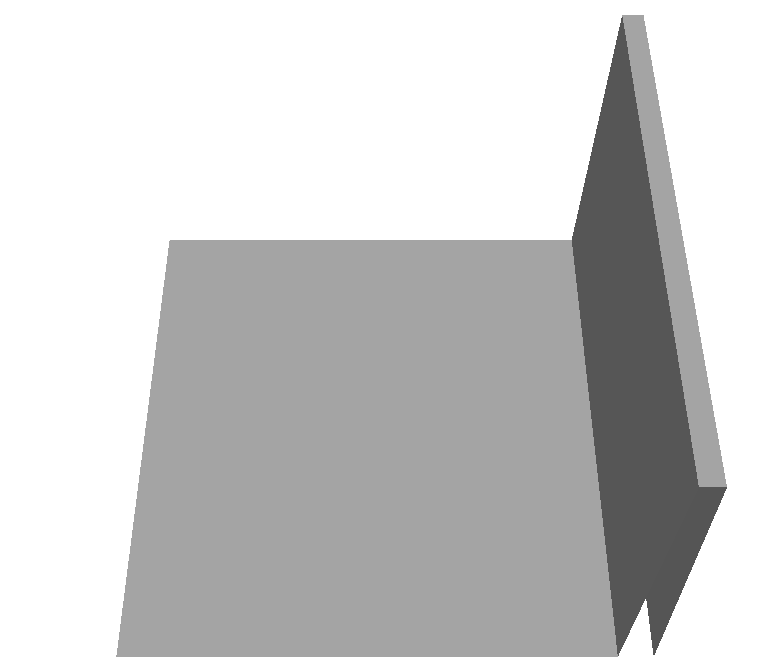
\includegraphics[width=\linewidth]{../img/5/custom_patches/walls_front/all/00-3d.png}
    \end{subfigure}
    \begin{subfigure}[b]{0.24\textwidth}
    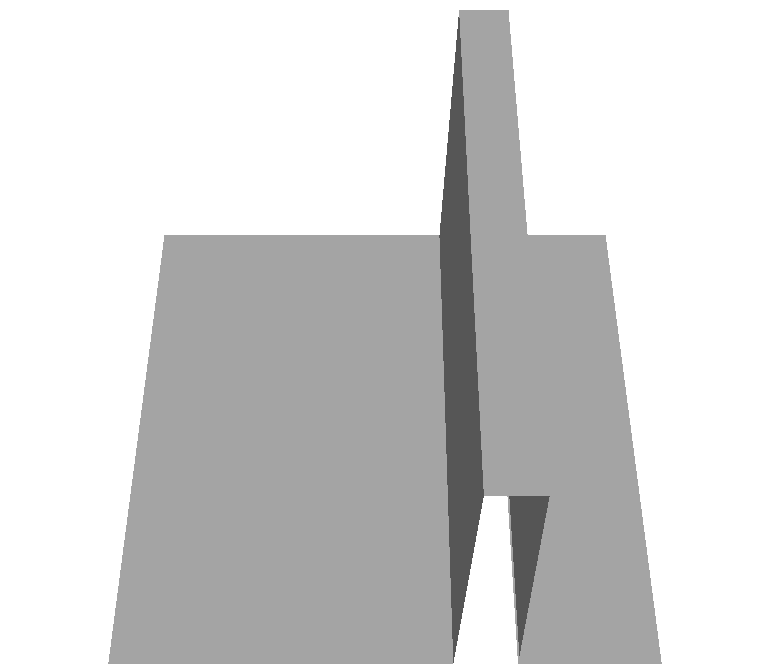
\includegraphics[width=\linewidth]{../img/5/custom_patches/walls_front/all/04-3d.png}
    \end{subfigure}
    \begin{subfigure}[b]{0.24\textwidth}
    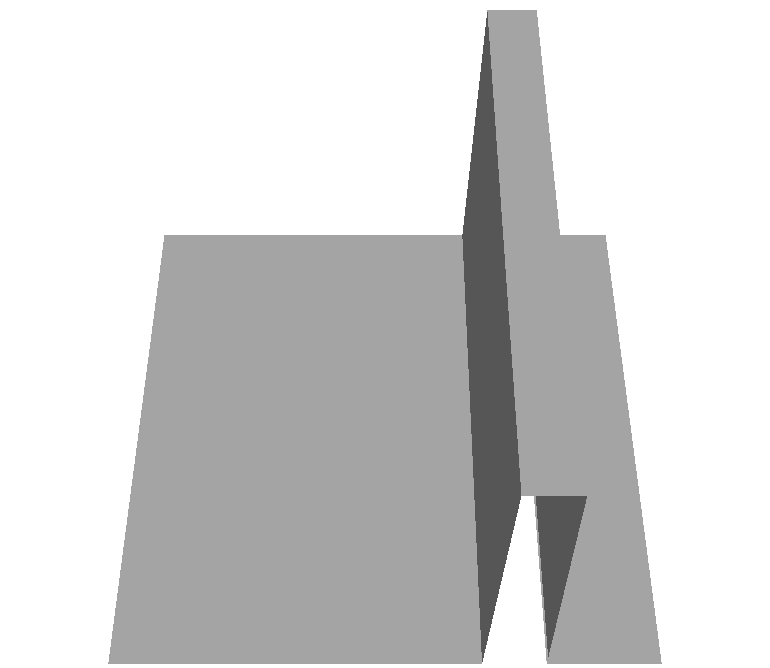
\includegraphics[width=\linewidth]{../img/5/custom_patches/walls_front/all/08-3d.png}
    \end{subfigure}
    \begin{subfigure}[b]{0.24\textwidth}
    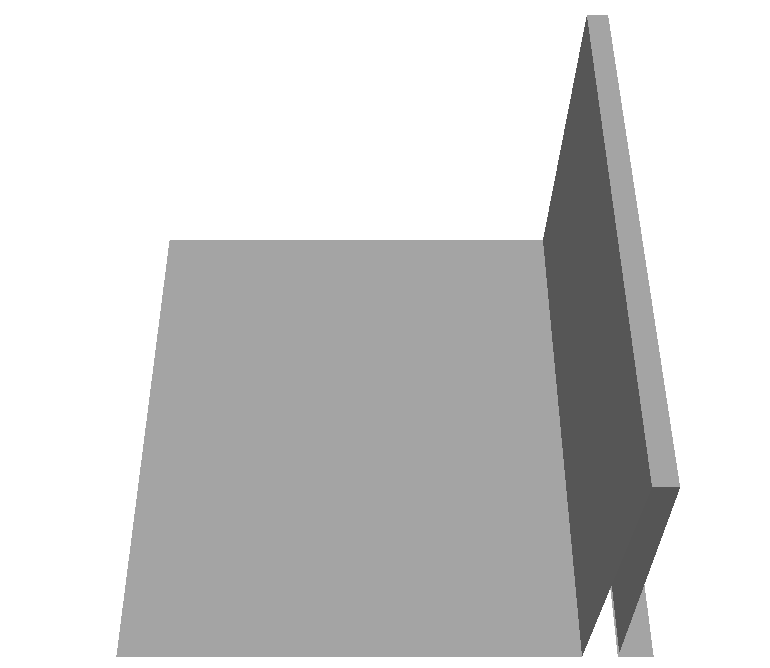
\includegraphics[width=\linewidth]{../img/5/custom_patches/walls_front/all/12-3d.png}
    \end{subfigure}
    \begin{subfigure}[b]{0.24\textwidth}
    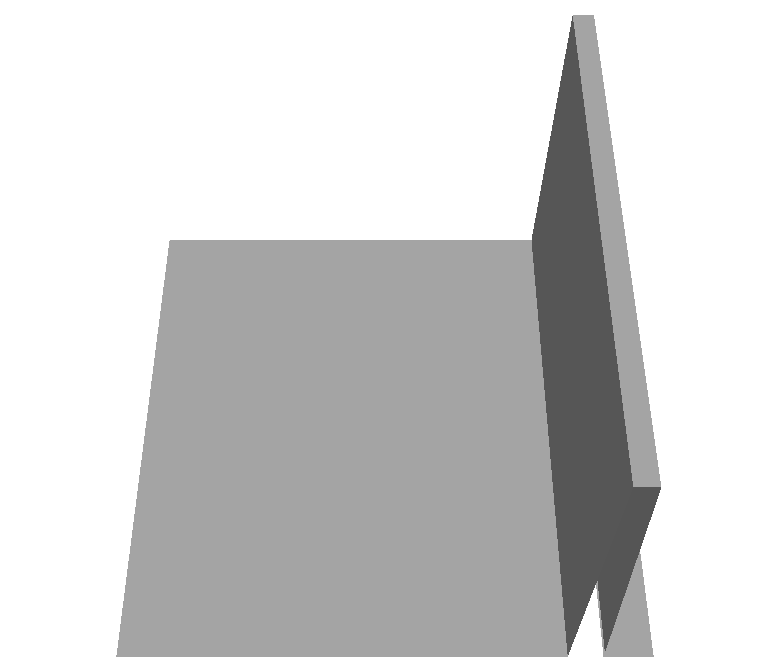
\includegraphics[width=\linewidth]{../img/5/custom_patches/walls_front/all/16-3d.png}
    \end{subfigure}
    \begin{subfigure}[b]{0.24\textwidth}
    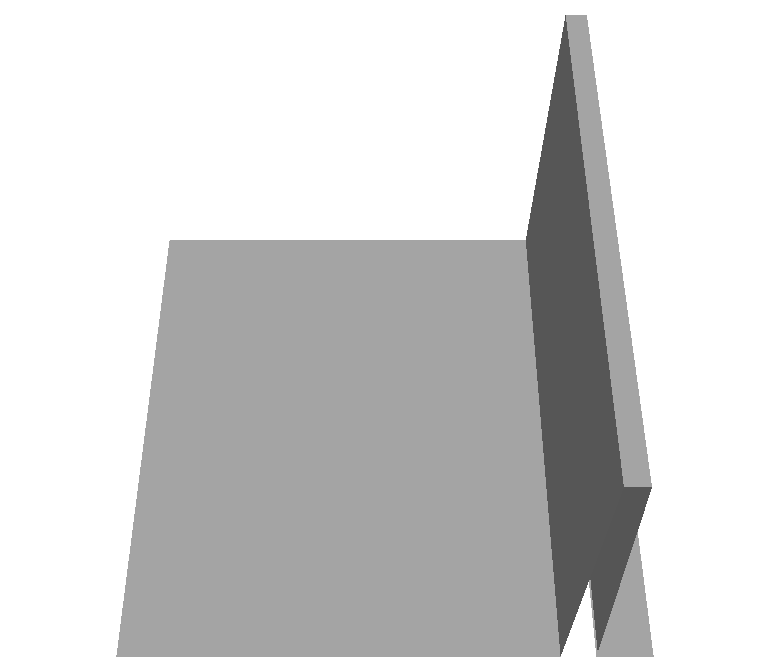
\includegraphics[width=\linewidth]{../img/5/custom_patches/walls_front/all/18-3d.png}
    \end{subfigure}
    \begin{subfigure}[b]{0.24\textwidth}
    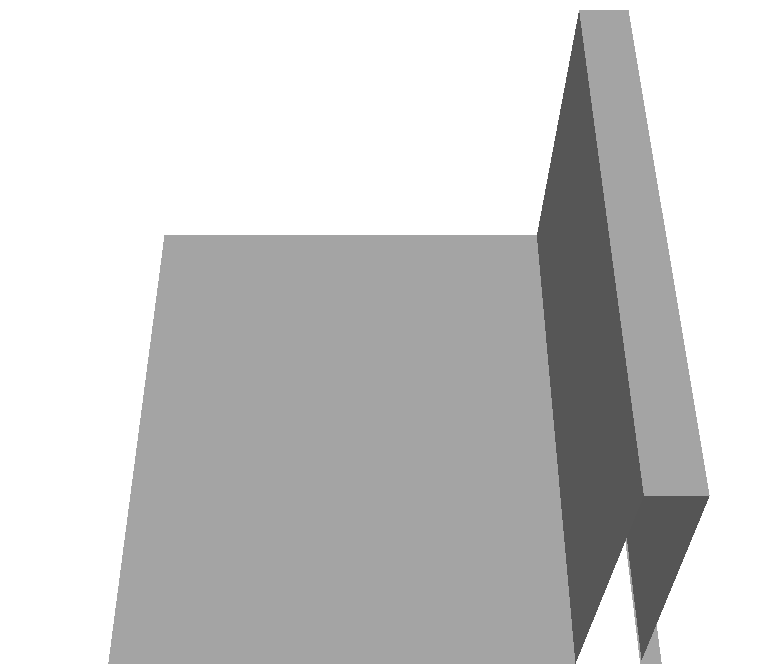
\includegraphics[width=\linewidth]{../img/5/custom_patches/walls_front/all/21-3d.png}
    \end{subfigure}
    \begin{subfigure}[b]{0.24\textwidth}
    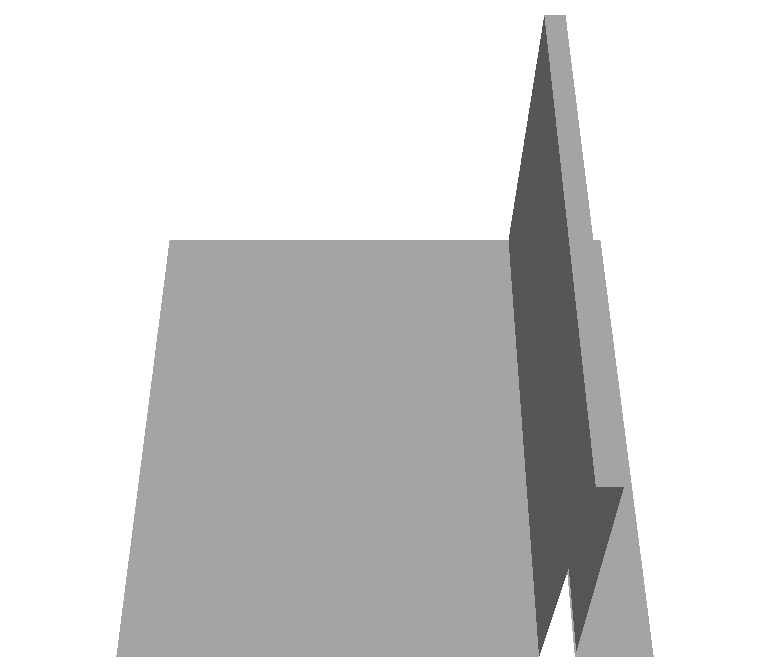
\includegraphics[width=\linewidth]{../img/5/custom_patches/walls_front/all/24-3d.png}
    \end{subfigure}
    \caption{Some of the tested patches with a non traversable walls at increasing distance from the robot.}
\label{fig: wall-distance}
    \end{figure}
The model's predictions are displayed in figure \ref{fig : wall-distance-preds}. We can see how the two classes invert their values around $20$cm. Moreover, the predictions, are consistent and do not change multiple times. Intuitively, if a wall is traversable from a certain distance, it will still be if we place even further.
\begin{figure}[htbp]
    \centering
\begin{subfigure}[b]{1\textwidth}
    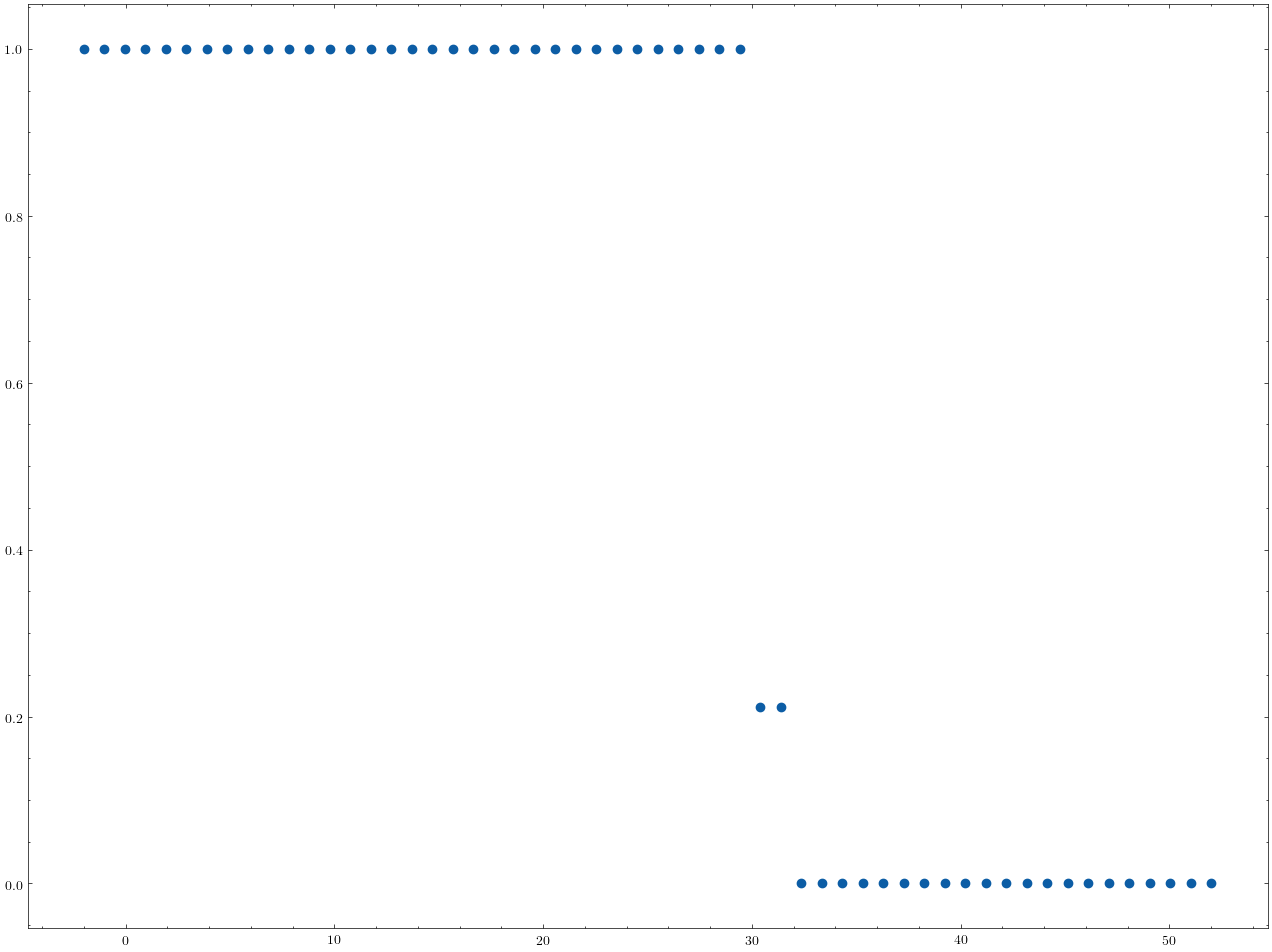
\includegraphics[width=\linewidth]{../img/5/custom_patches/walls_front/predictions.png}
    \end{subfigure}
    \caption{Traversability probabilities for patches  with a non traversable walls at increasing distance from the robot.}
\label{fig  : wall-distance-preds}
\end{figure}
% Summarized by the following table:
% \begin{table} [htbp]
%     \centering
%     \begin{tabular}{l|cc}
%         Distance(cm) & Prediction \\ 
%         \hline
%         0 - 20  & Not traversable \\ 
%         22 - end & Traversable \\ 
%         \hline
%     \end{tabular}
%     \caption{Model predictions for patches  with a non traversable walls at increasing distance from the robot.}
% \end{table}
To be sure the results are correct, we run the last not traversable and the first traversable patch on the simulator to get real advancement. In the simulator, Krock advances $18.3$cm on the first, not traversable patch \ref{fig : walls-traversable-a} where the wall is at $20$cm from the robot's head. While, on the first traversable patch, figure ref{fig :walls-traversable-b}, with a wall at $22$cm, the robot was able to travel for $20.2$cm. Correctly, the network's predictions are supported by the ground truth obtained from the simulation. Even more important, the model understood that the distance from the obstacle is more relevant than its height.
\begin{figure}[htbp]
    \centering
    \begin{subfigure}[b]{0.33\textwidth}
        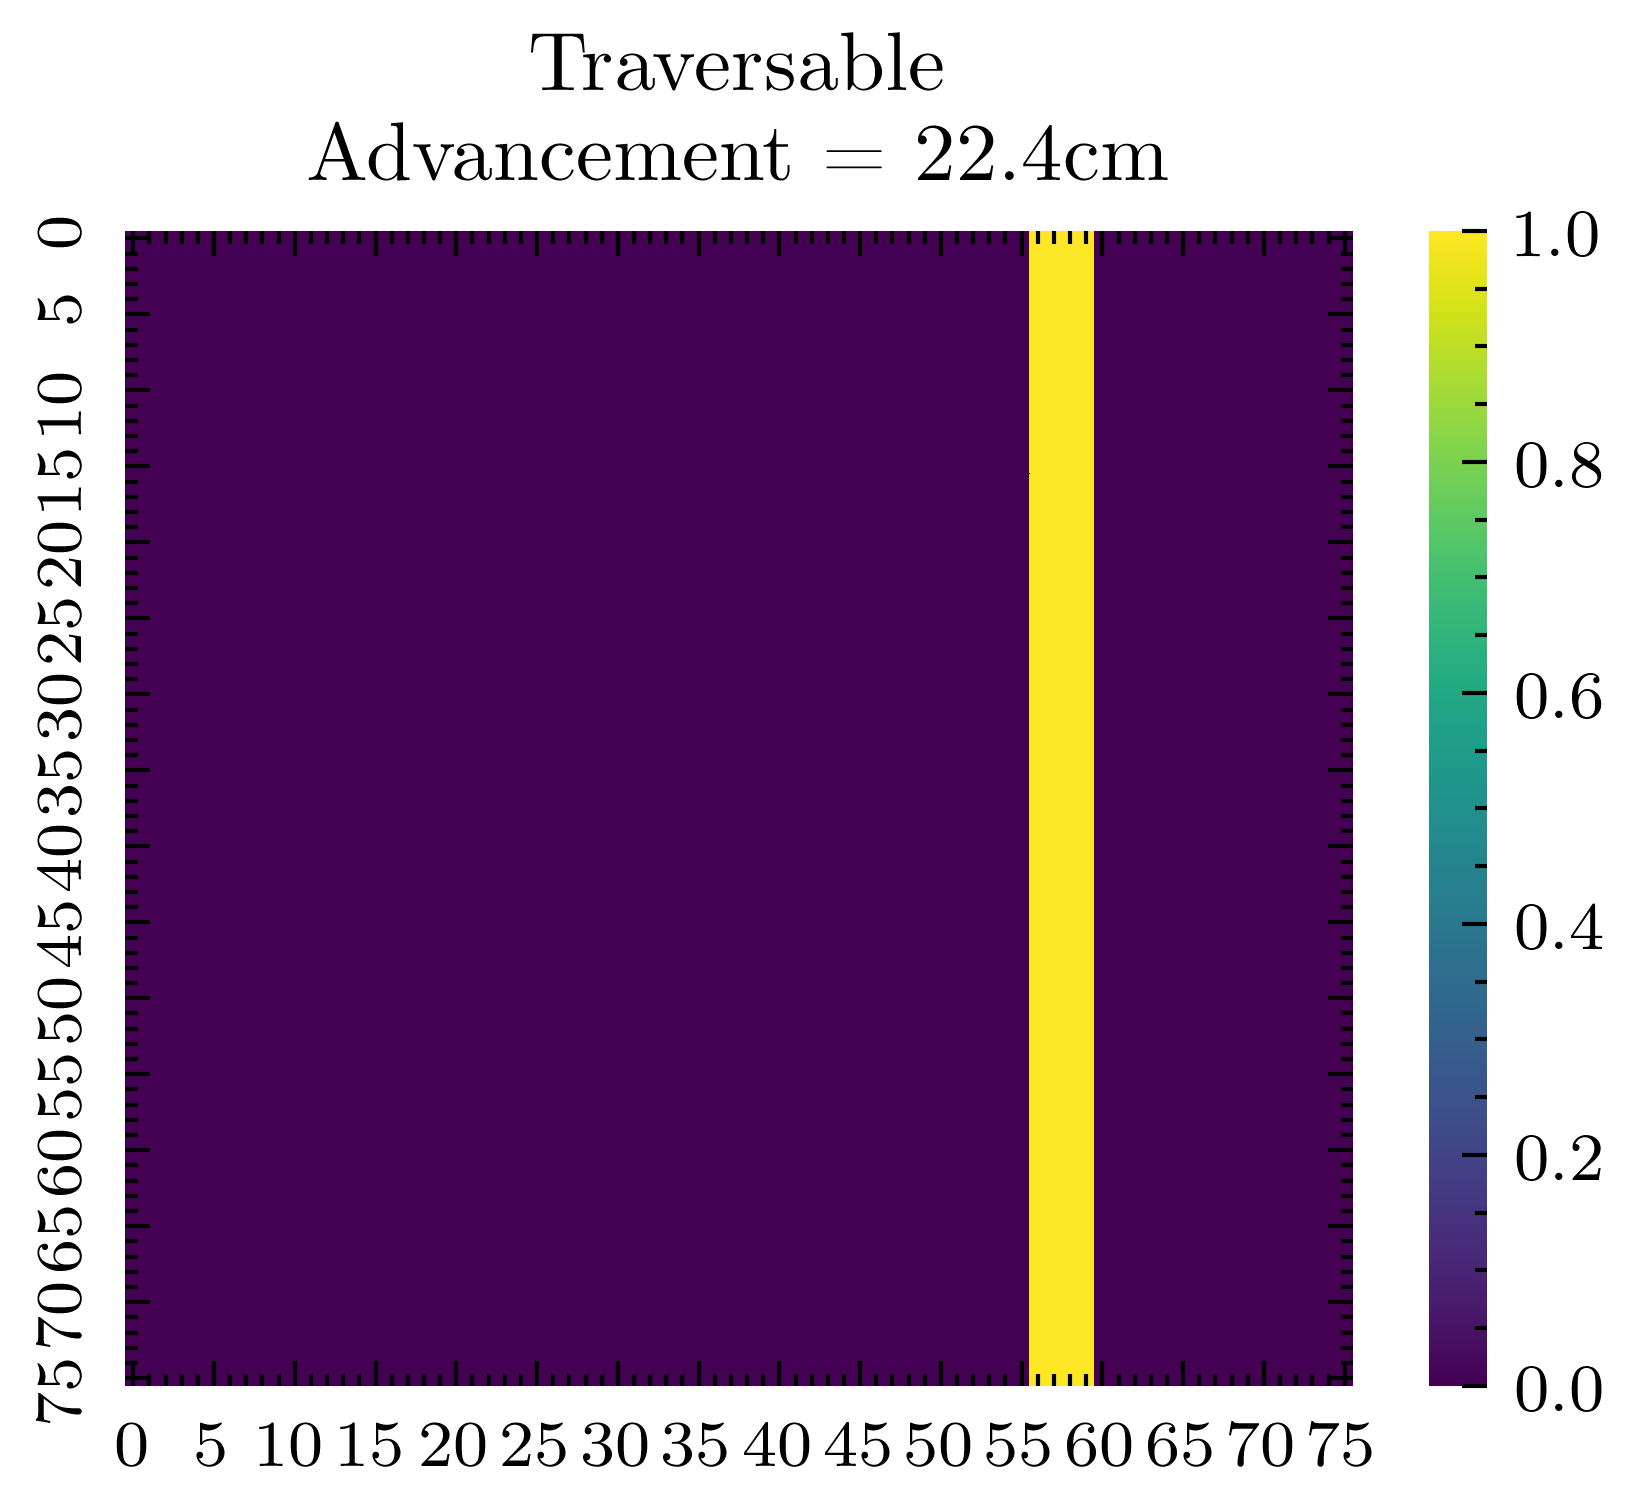
\includegraphics[width=\linewidth]{../img/5/custom_patches/walls_front/2-2d.png}
        \end{subfigure}   
    \begin{subfigure}[b]{0.33\textwidth}
        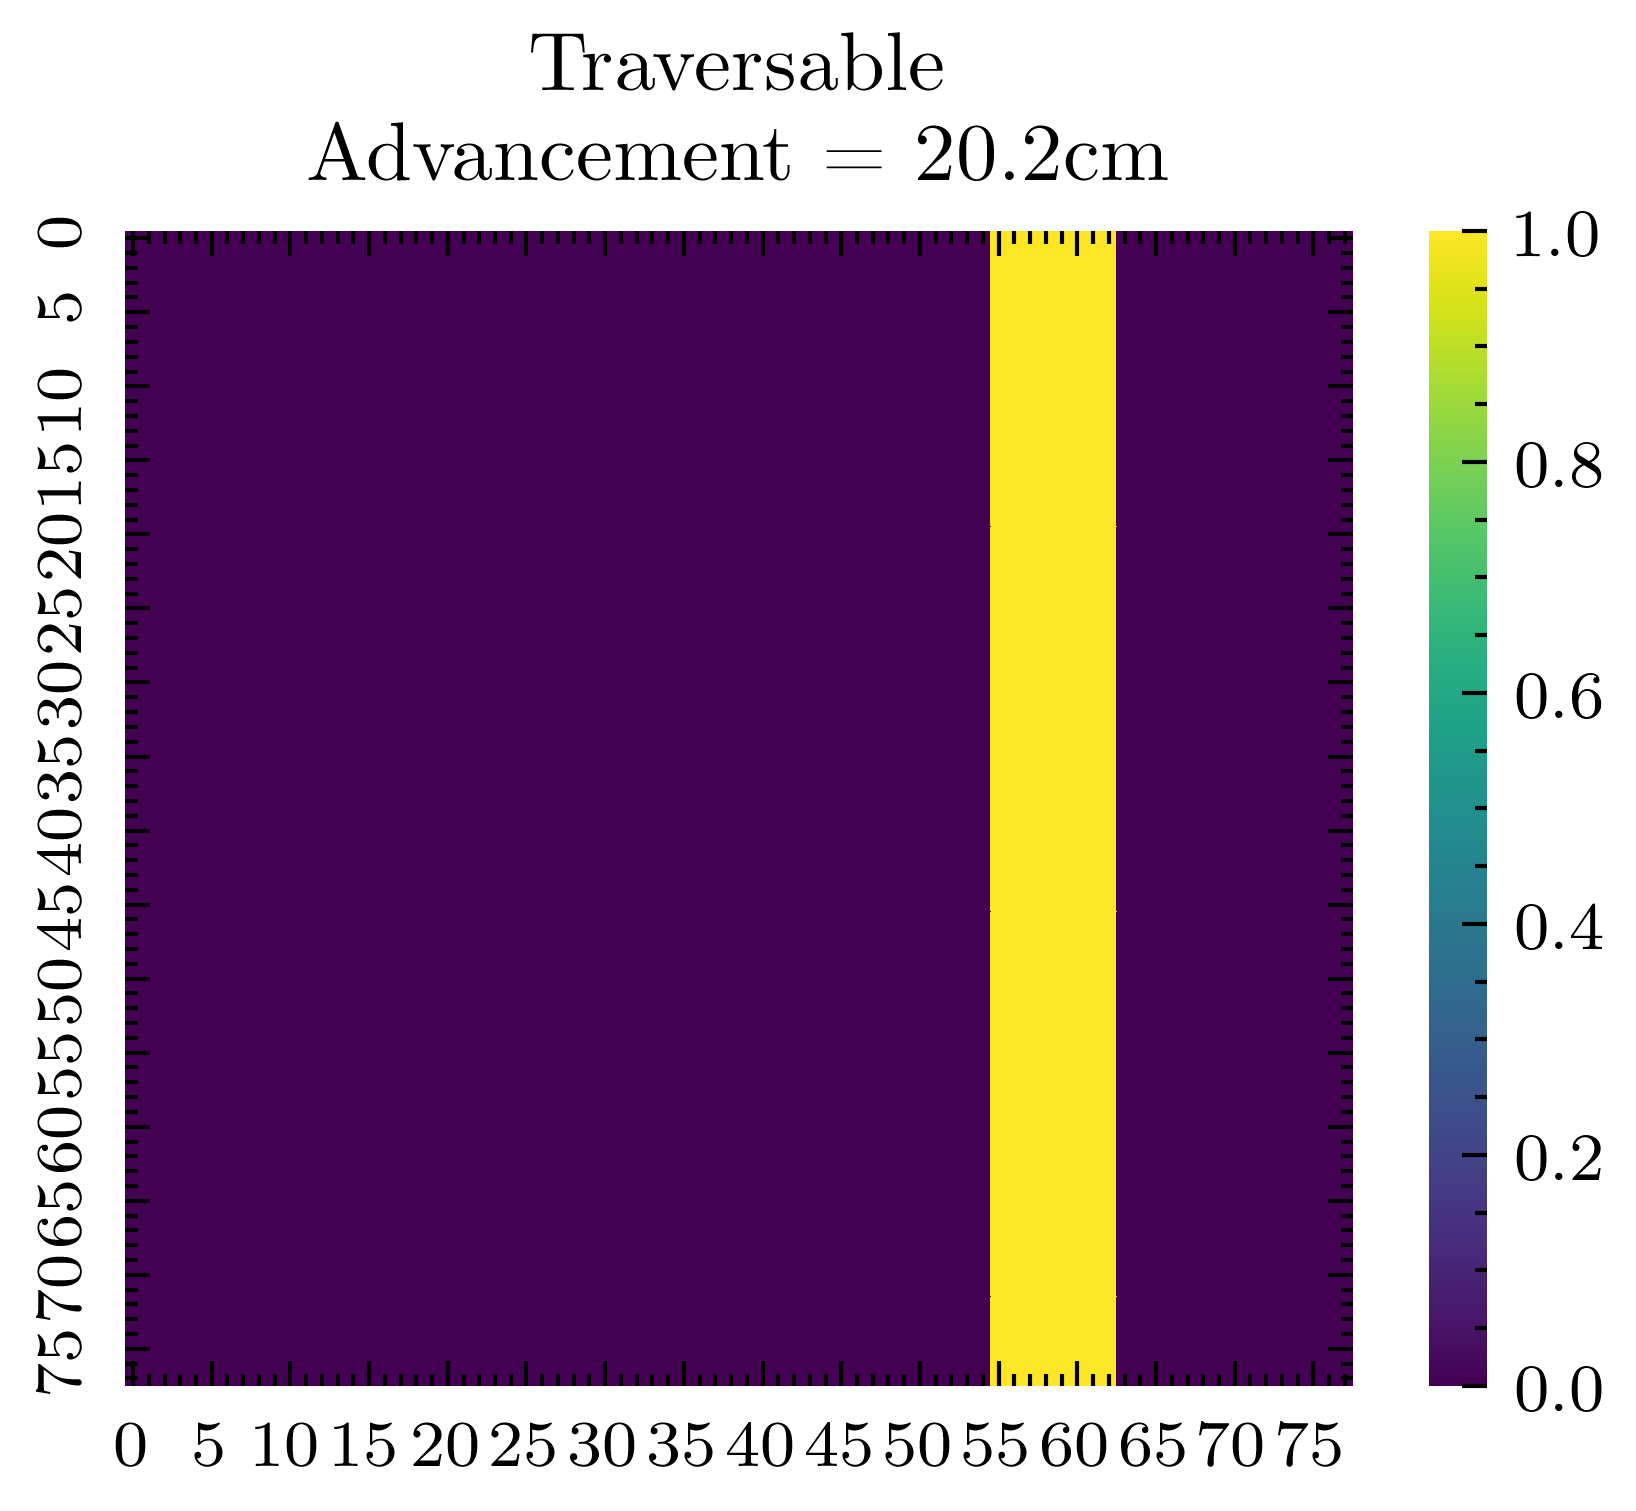
\includegraphics[width=\linewidth]{../img/5/custom_patches/walls_front/1-2d.png}
    \end{subfigure}   \\
    \begin{subfigure}[b]{0.33\textwidth}
        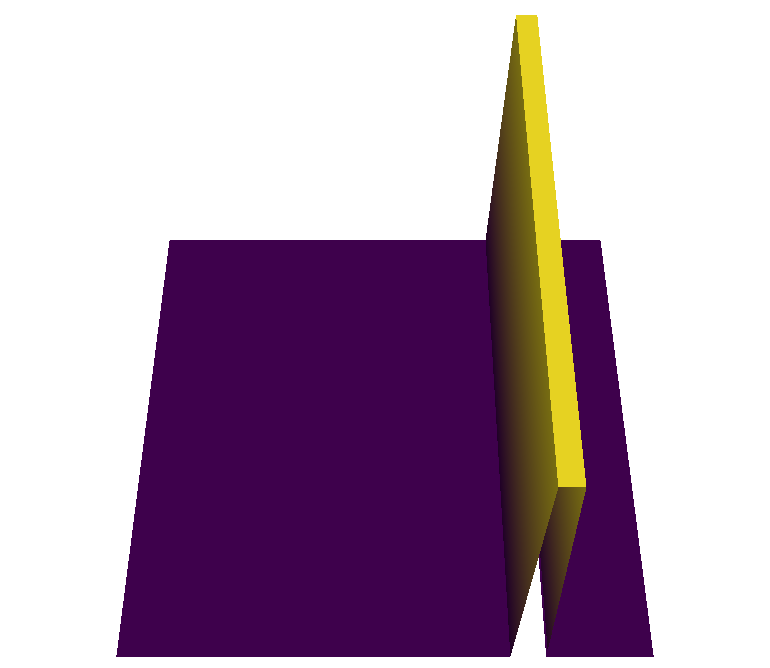
\includegraphics[width=\linewidth]{../img/5/custom_patches/walls_front/2-3d.png}
        \caption{Distance $20$cm}
    \label{fig: walls-traversable-a}
    \end{subfigure}   
    \begin{subfigure}[b]{0.33\textwidth}
        
\includegraphics[width=\linewidth]{../img/5/custom_patches/walls_front/1-3d.png}
        \caption{Distance $22$cm}
    \label{fig: walls-traversable-b}
    \end{subfigure}   
    \caption{We run the last and first not traversable and traverable patch labeled by the model. Correctly, the real advancement is greater than the threshold when the distance between the robot is also greater.}
    \label{fig: walls-traversable}
\end{figure}
Furthermore, we increased the wall size of the first traversable patch, figure \ref{fig : walls-traversable-b}, to $10$ and to $50$m to see if the model will be confused. Accurately, the robot was not confused by the enourmous wall and the predictions did no change and those patches were still labeled as traversable. Figure \ref{fig : walls-tall} visualize those patches.
\begin{figure}[htbp]
    \centering
    \begin{subfigure}[b]{0.33\textwidth}
        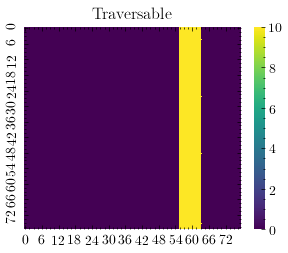
\includegraphics[width=\linewidth]{../img/5/custom_patches/walls_front/big-1-2d.png}
    \caption{height $=10$m}
    \end{subfigure}   
    \begin{subfigure}[b]{0.33\textwidth}
        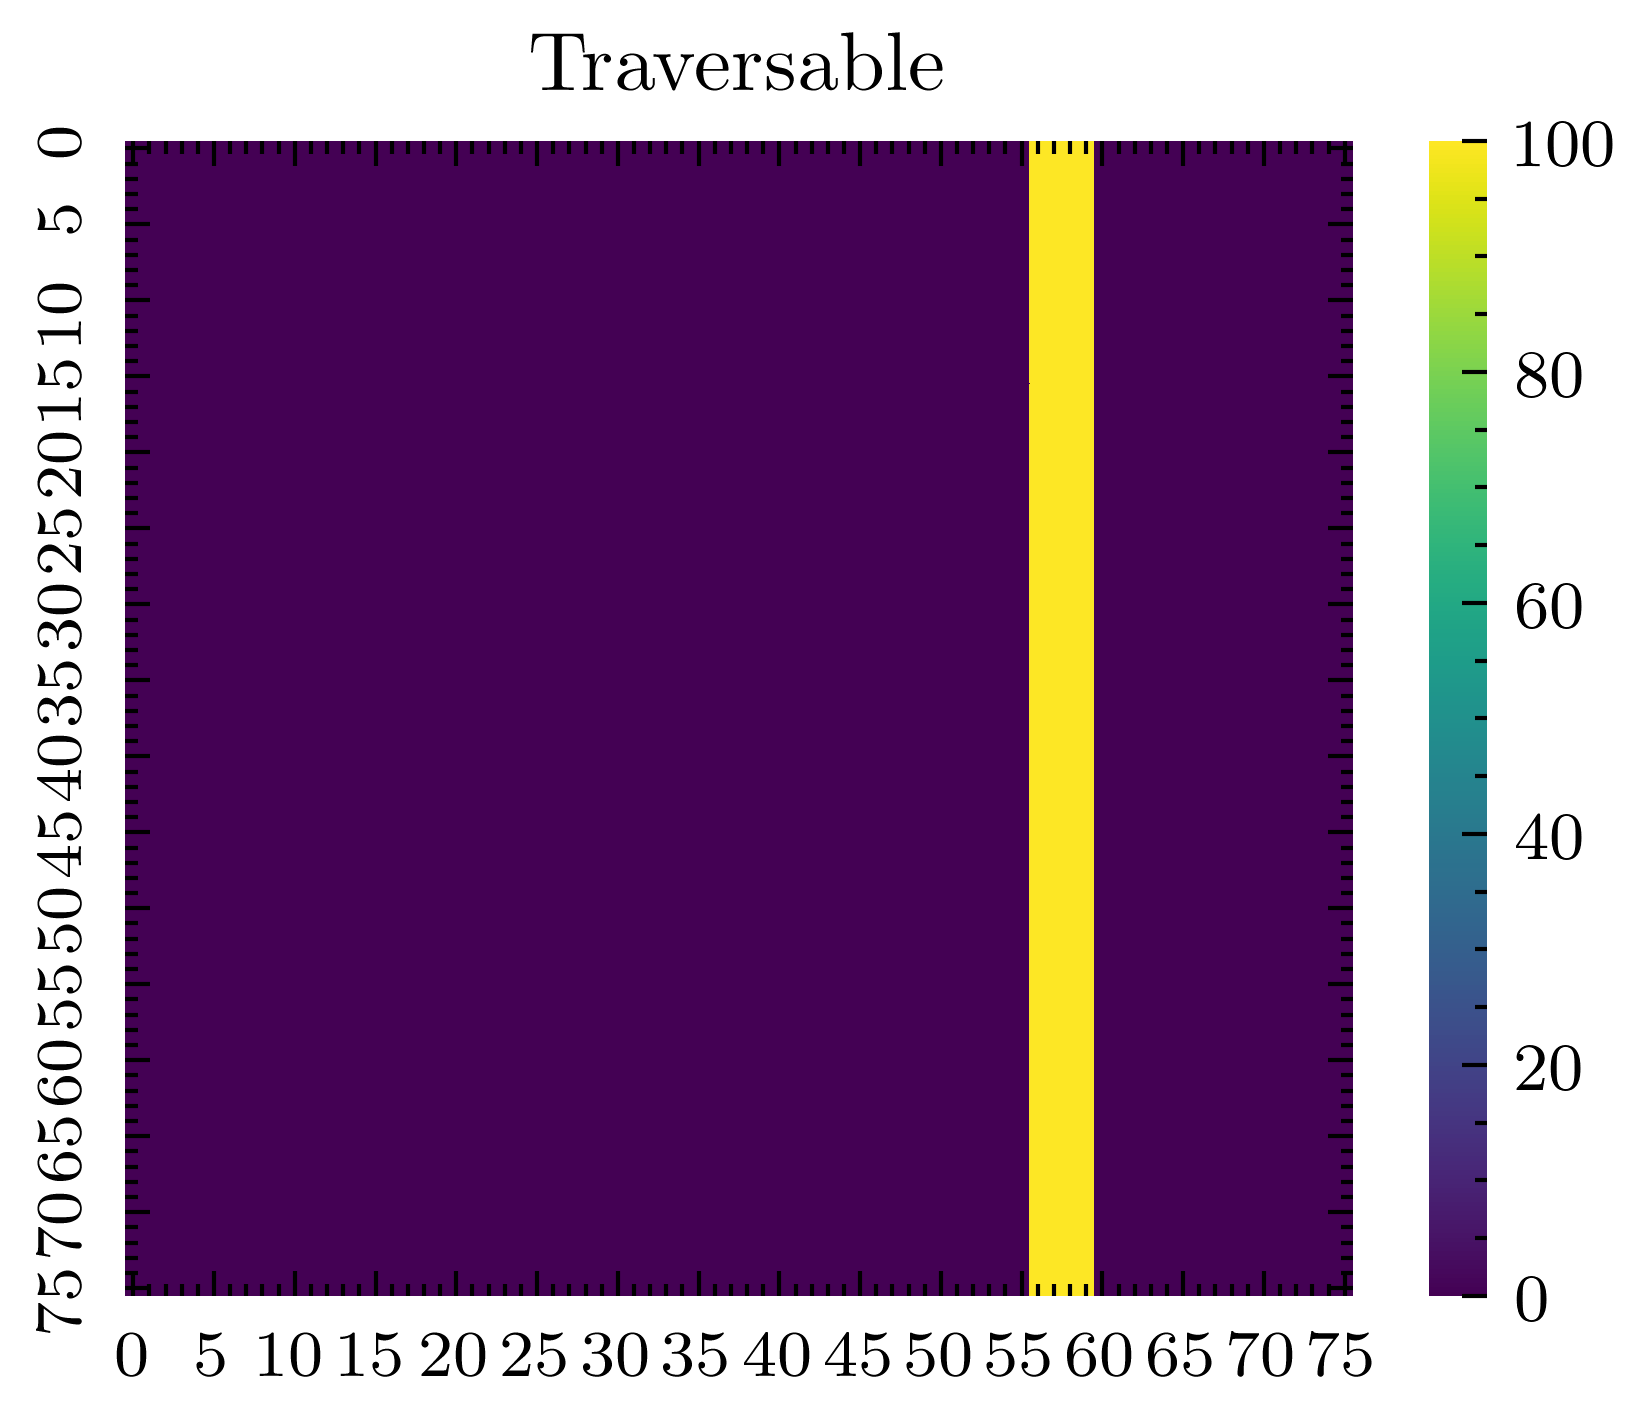
\includegraphics[width=\linewidth]{../img/5/custom_patches/walls_front/big-2-2d.png}
        \caption{height $=50$m}
    \end{subfigure}   
\caption{Two patches with a very tall wall at a distance major than the threshold. The model labels them as traversable without been confused by the huge obstacle.}    
\label{fig : walls-tall}
\end{figure}
\subsection{Increasing height walls ahead}
After we tested the distance from Krock's and a wall, we decided to fix the obstacle position but increase its heights.  We run forty patches in the simulator with a wall place exactly in front of the robot with height from $1$cm to $20$cm. Figure \ref{fig :walls-height} shows some of the inputs.

\begin{figure}[htbp]
    \centering
    \begin{subfigure}[b]{0.24\textwidth}
    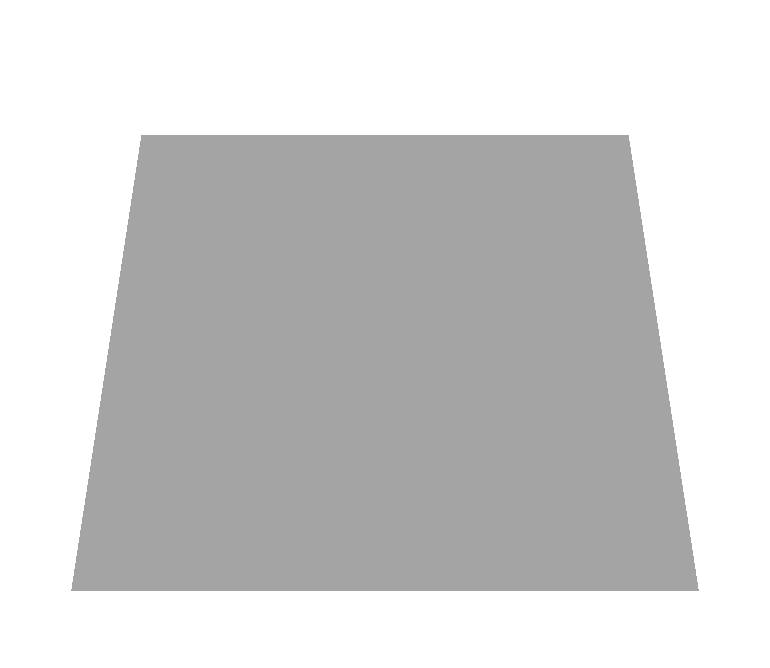
\includegraphics[width=\linewidth]{../img/5/custom_patches/walls_increasing/all/00-3d.png}
    \end{subfigure}
    \begin{subfigure}[b]{0.24\textwidth}
    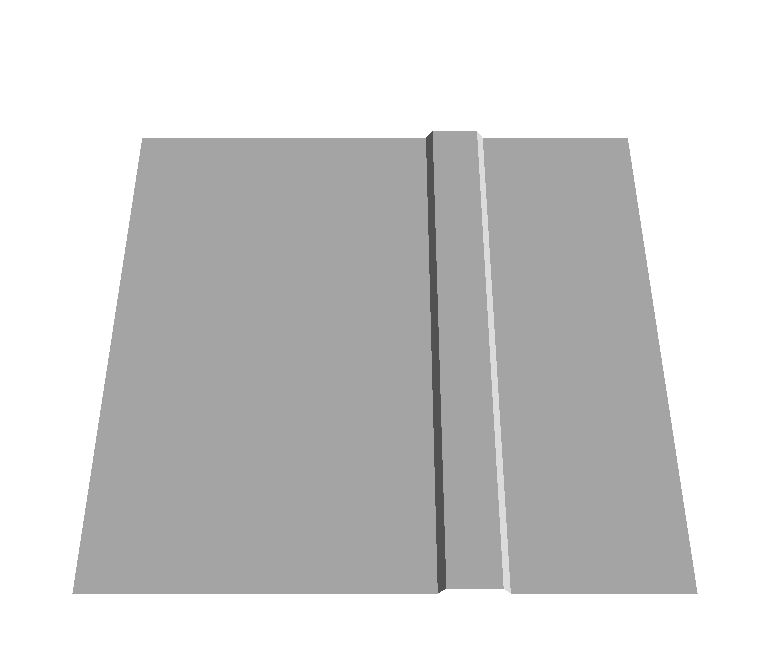
\includegraphics[width=\linewidth]{../img/5/custom_patches/walls_increasing/all/03-3d.png}
    \end{subfigure}
    \begin{subfigure}[b]{0.24\textwidth}
    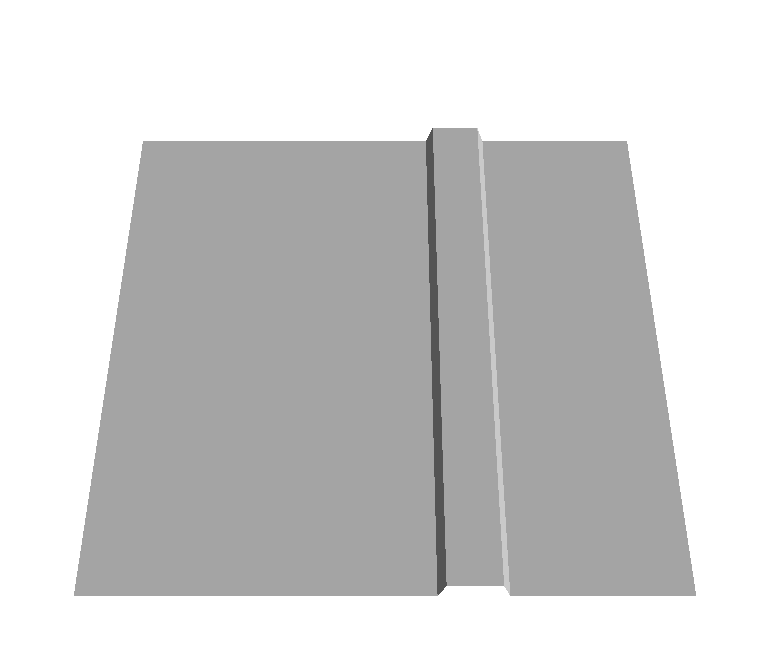
\includegraphics[width=\linewidth]{../img/5/custom_patches/walls_increasing/all/06-3d.png}
    \end{subfigure}
    \begin{subfigure}[b]{0.24\textwidth}
    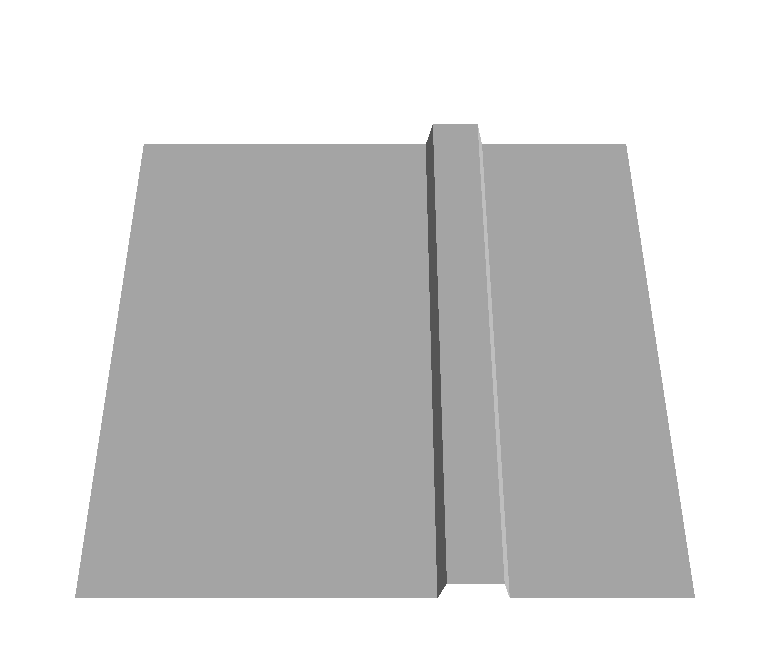
\includegraphics[width=\linewidth]{../img/5/custom_patches/walls_increasing/all/09-3d.png}
    \end{subfigure}
    \begin{subfigure}[b]{0.24\textwidth}
    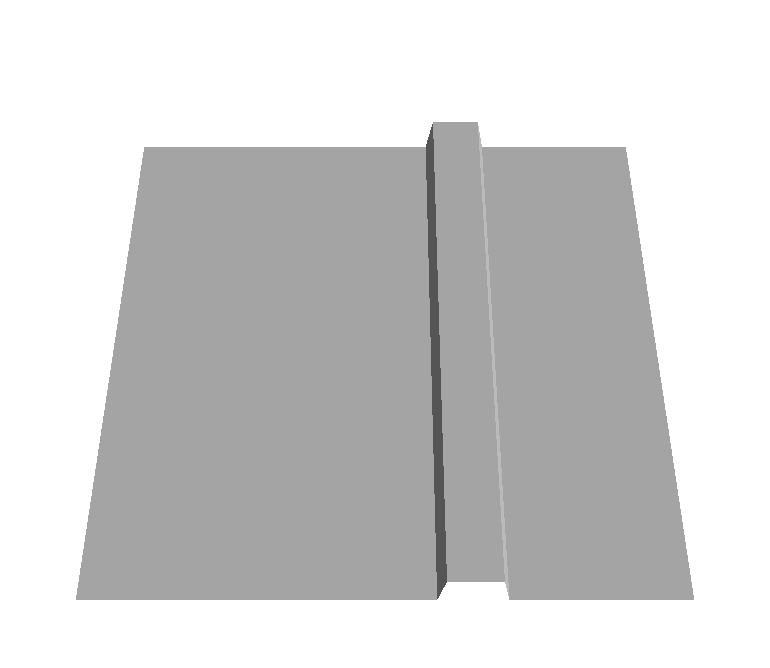
\includegraphics[width=\linewidth]{../img/5/custom_patches/walls_increasing/all/11-3d.png}
    \end{subfigure}
    \begin{subfigure}[b]{0.24\textwidth}
    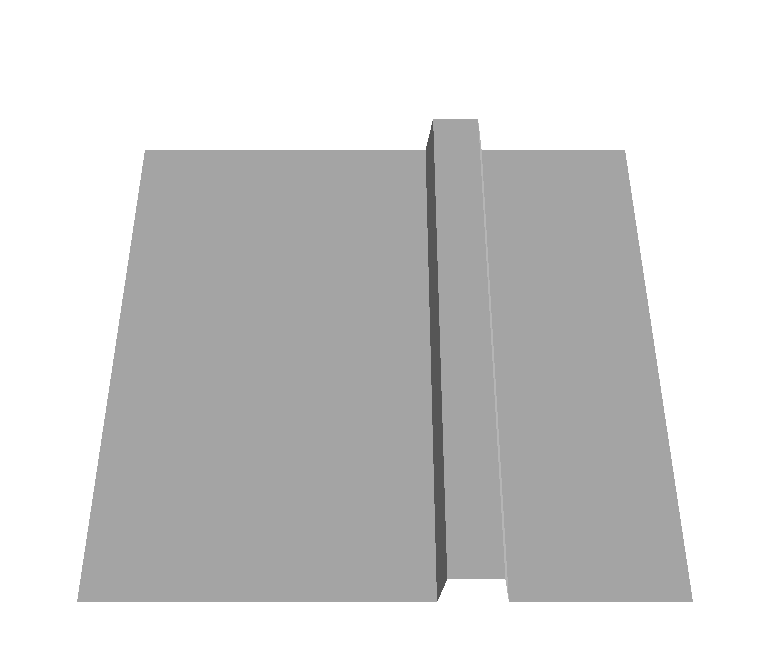
\includegraphics[width=\linewidth]{../img/5/custom_patches/walls_increasing/all/14-3d.png}
    \end{subfigure}
    \begin{subfigure}[b]{0.24\textwidth}
    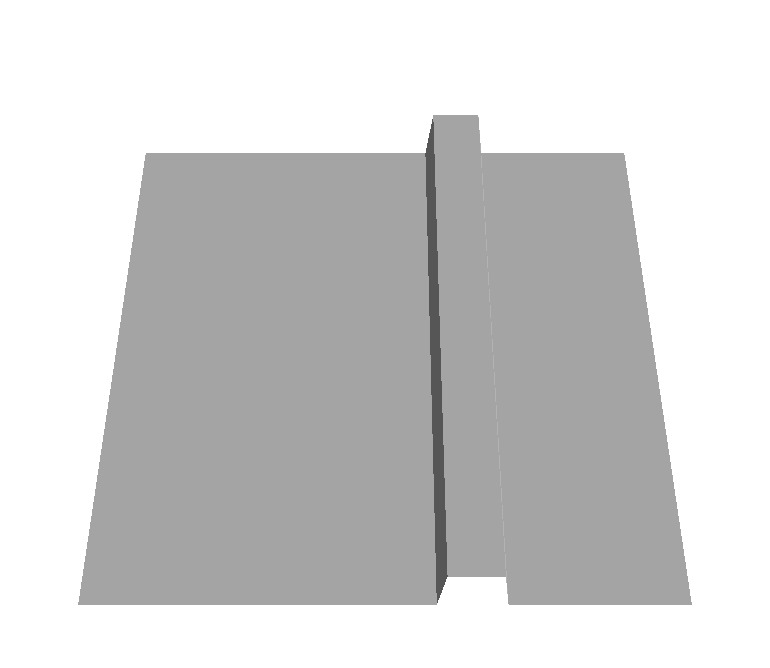
\includegraphics[width=\linewidth]{../img/5/custom_patches/walls_increasing/all/17-3d.png}
    \end{subfigure}
    \begin{subfigure}[b]{0.24\textwidth}
    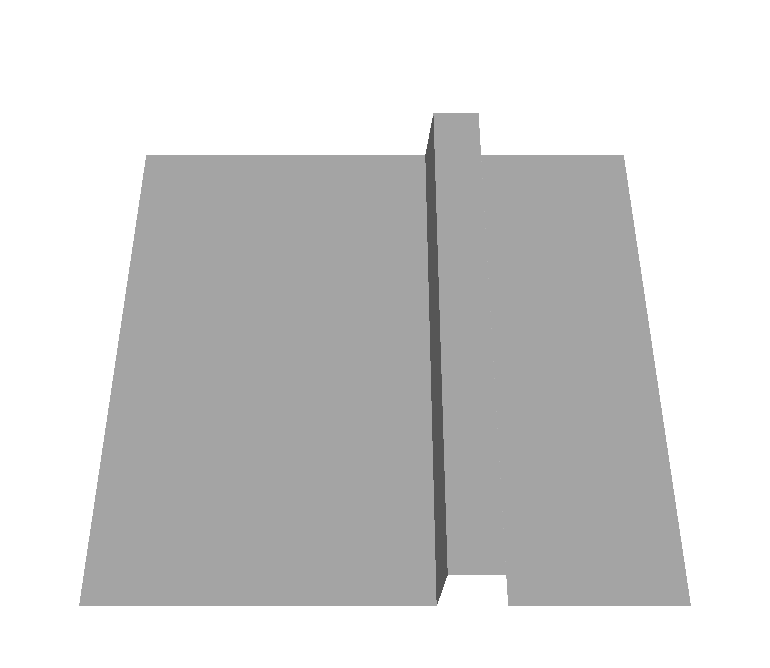
\includegraphics[width=\linewidth]{../img/5/custom_patches/walls_increasing/all/19-3d.png}
    \end{subfigure}
    \caption{Some of the tested patches with a walls at increasing height ahead of Krock.}
\label{fig : walls-height}
    \end{figure}
The models predicted that the walls under $10$cm are traversable. We plotted the classes probabilities in figure \ref{fig : walls-height-preds} in which we see that in the edge case, $\approx 10$cm, the model's prediction change smoothly revealing a degree of uncertainty, positively the estimator outputs to change smoothly.
\begin{figure}[htbp]
    \centering
\begin{subfigure}[b]{1\textwidth}
    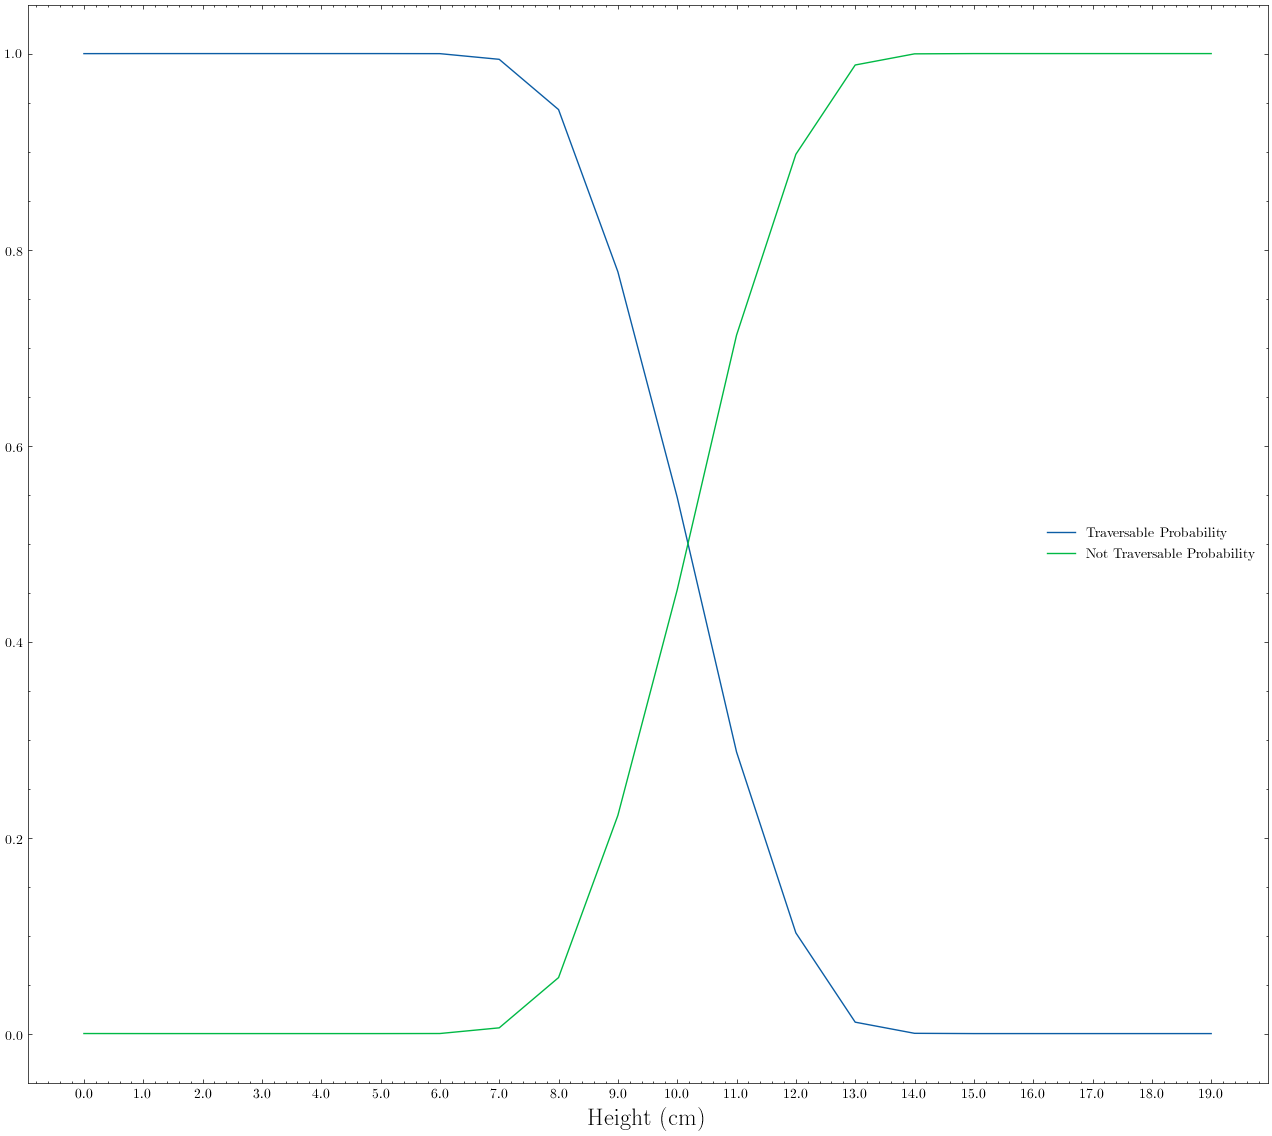
\includegraphics[width=\linewidth]{../img/5/custom_patches/walls_increasing/predictions.png}
    \end{subfigure}
    \caption{Traversability probabilities against walls height in front of Krock.}
\label{fig : walls-height-preds}
\end{figure}
We compared the model's prediction with the advancement computed in the simulator using the same approach from the last section. Figure \ref{fig: wall-height-sim} shows the results from the last traversable patch and the first non traversable.

\begin{figure}[htbp]
    \centering
    \begin{subfigure}[b]{0.33\textwidth}
        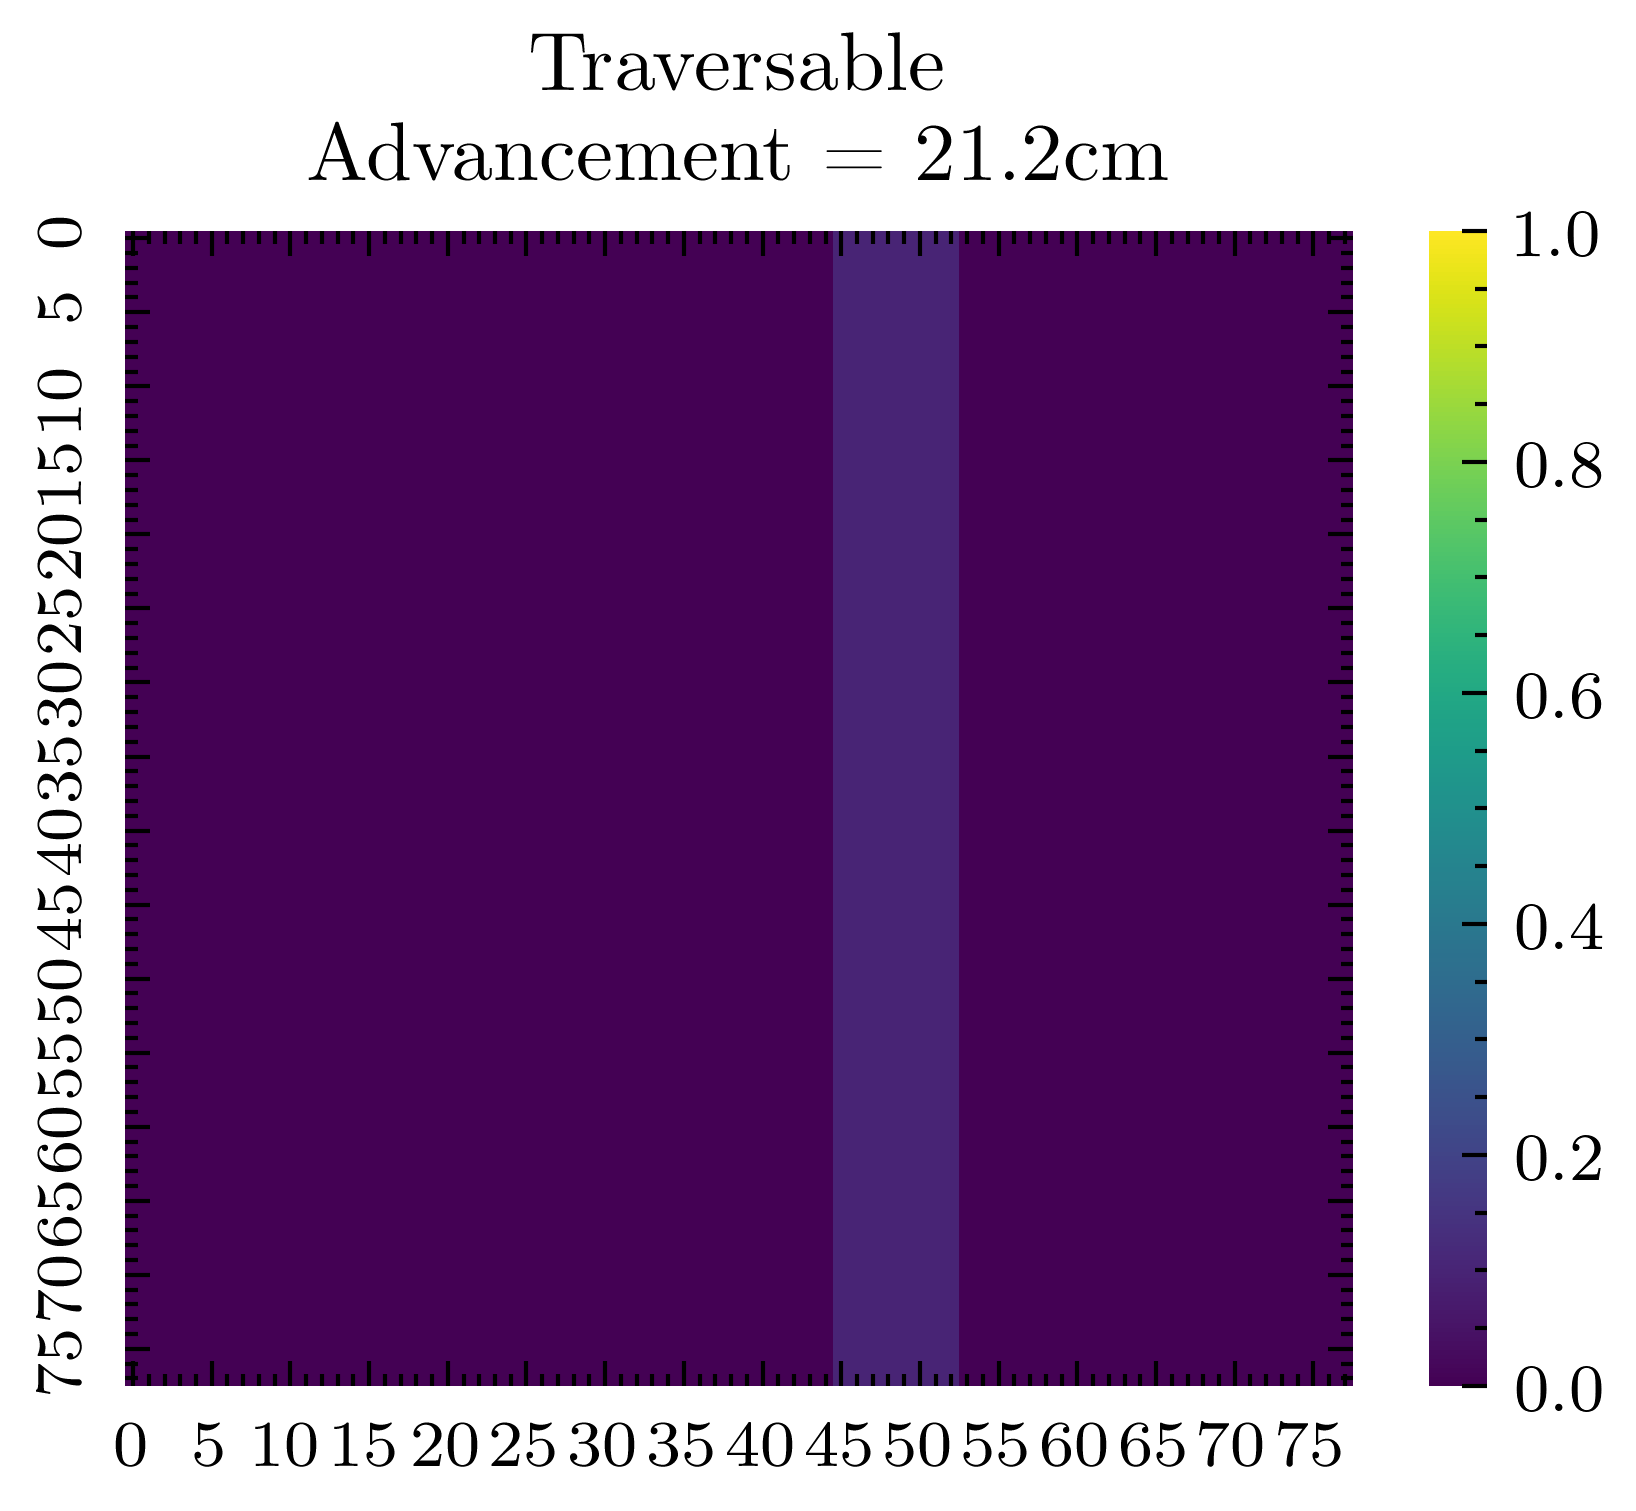
\includegraphics[width=\linewidth]{../img/5/custom_patches/walls_increasing/1-2d.png}
    \end{subfigure}   
    \begin{subfigure}[b]{0.33\textwidth}
        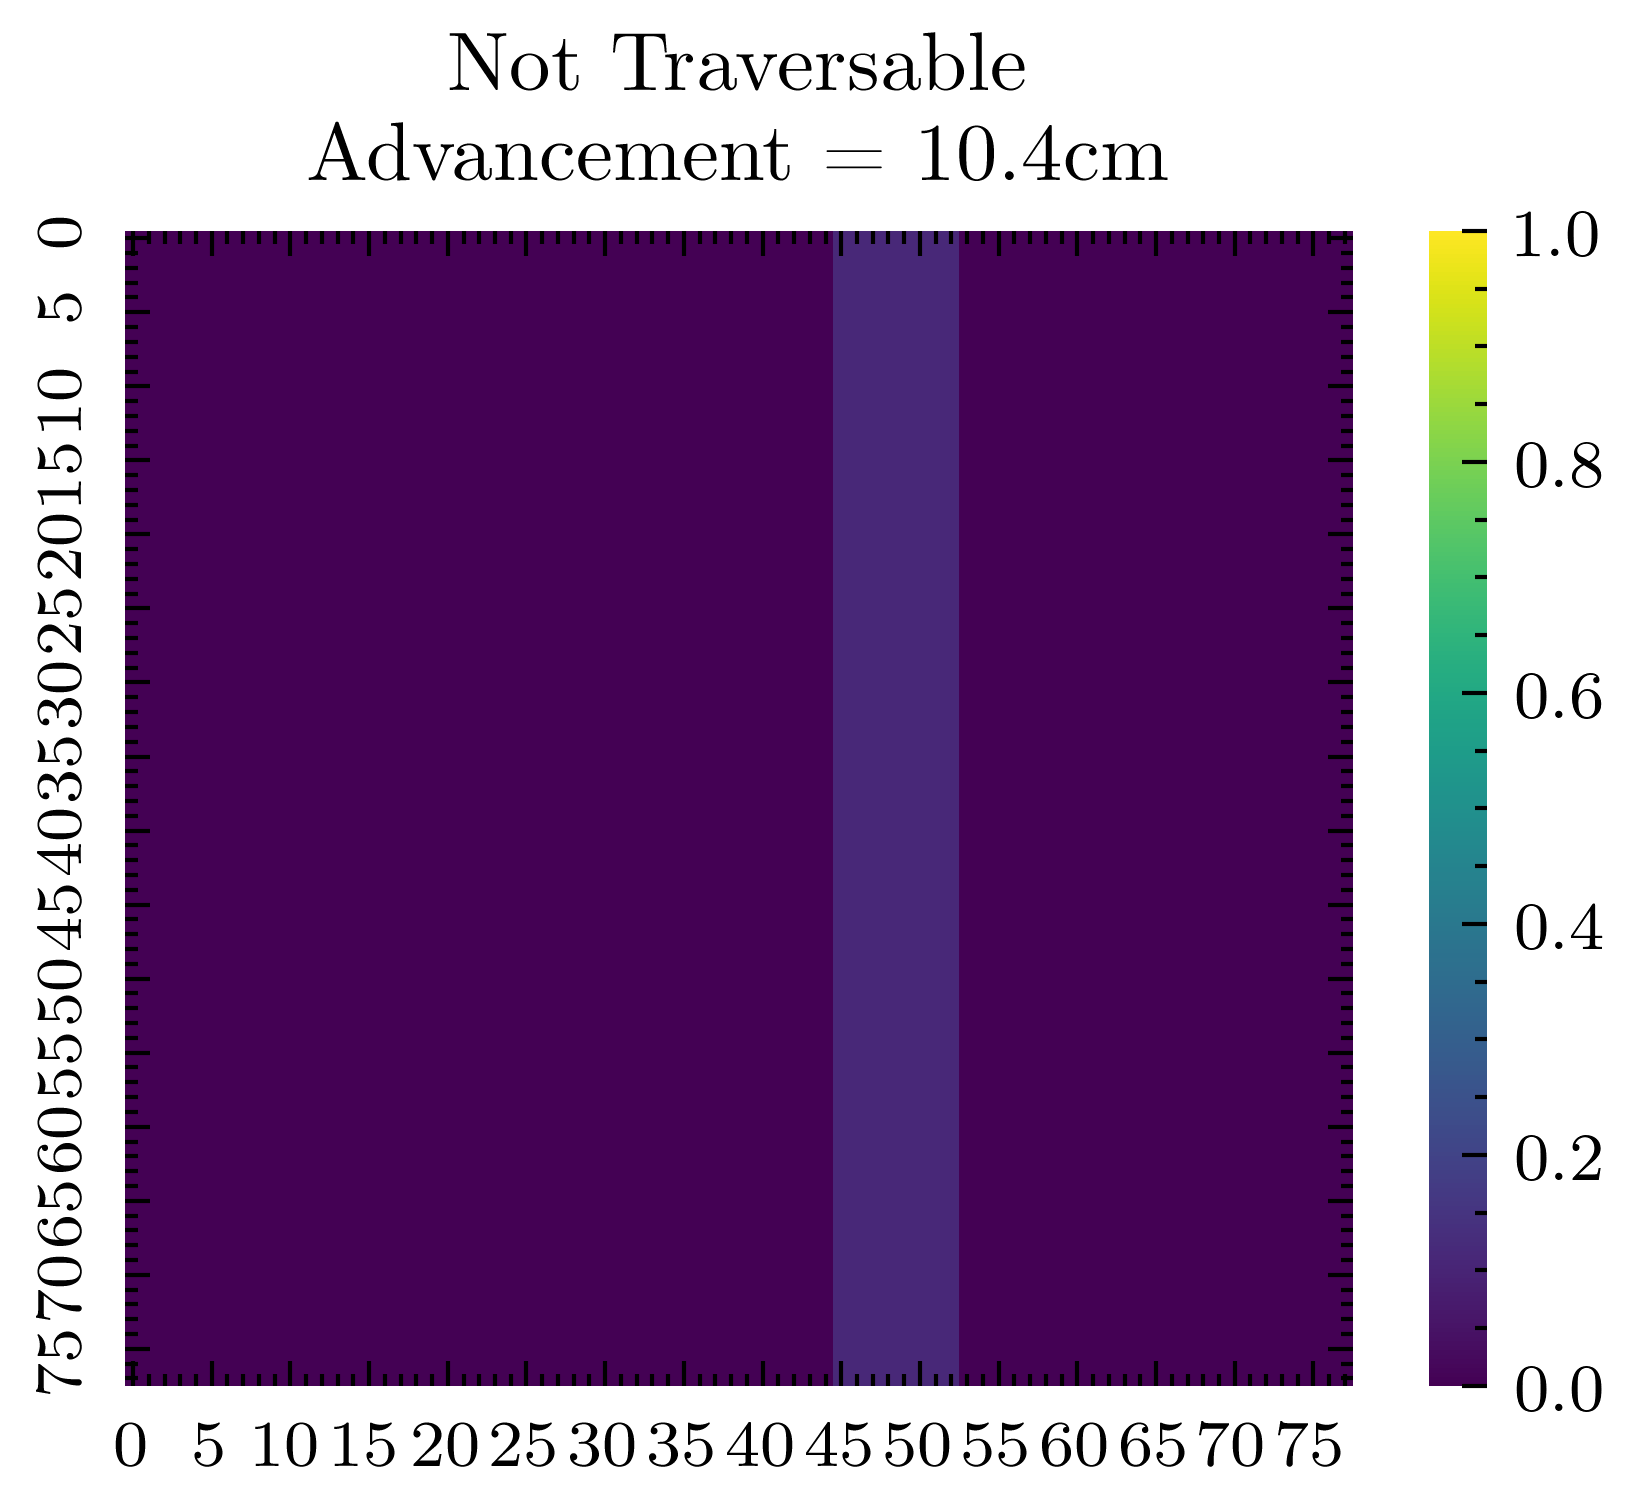
\includegraphics[width=\linewidth]{../img/5/custom_patches/walls_increasing/2-2d}
    \end{subfigure}   
    \begin{subfigure}[b]{0.33\textwidth}
        
\includegraphics[width=\linewidth]{../img/5/custom_patches/walls_increasing/1-3d.png}
    \caption{height $9$cm}
    \end{subfigure}   
    \begin{subfigure}[b]{0.33\textwidth}
        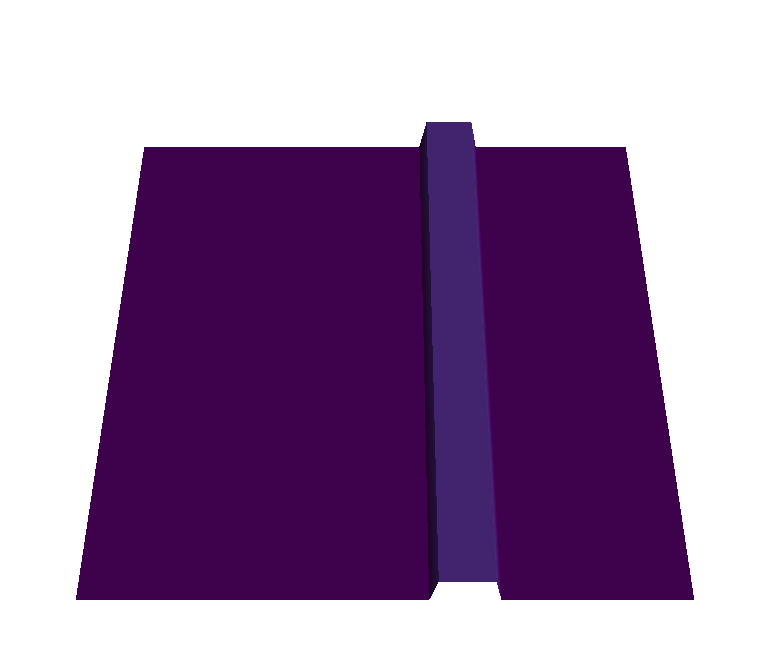
\includegraphics[width=\linewidth]{../img/5/custom_patches/walls_increasing/2-3d}
        \caption{Height $10$cm}
    \end{subfigure}   
    \caption{We run the last and first traversable and not traverable patch labeled by the model. Correctly the model's prediction matches the advancement from the simulator.} 
    \label{fig : wall-height-sim}
\end{figure}
In the first case, the simulator outputted and advancement of $21.2$cm meaning that Krock was able to overcome the obstacle, while it failed in the second case. Correctly, the predictions matched the real data.

\subsection{Increasing height and distance walls ahead.}
We combined the previous experiments and tested the model predictions against the ground truth for each height/distance combination. To reduce the number of samples and improve readability, we limited to consider only patches with a wall tall between $5$cm and $20$cm, we know from previous sections patches with a value smaller and bigger obstacle are traversable and not traversable respectively. Similar, we set the wall's distance from Krock's head between $1$cm to $30$cm for the same reasons. To evaluate the model's prediction, we run all the patches several times on the simulator and average the results. Figure \ref{fig:  walls-heights-preds} shows the models outputs. We highlighted the false positive and the false negative by red and blue respectively.  Since we spawned the robot directly on the patch inside the simulator, the outputs may change across different runs. Sometimes, two runs on the same patch can produce slighty different advancement due to some really small changes in the initial position of the robot caused the spawning procedure or some lag. Figure \ref{fig : walls-heights-advs} displays the real advancements average across six different runs for all the patches. Additionally, for completeness, we also display in figure \ref{fig: walls-heights-std} the variance between all simulation's runs to highlighted cases where the advancement changes the most across different runs:  

\begin{figure}[htbp]
    \centering
    \begin{subfigure}[b]{0.48\linewidth}
        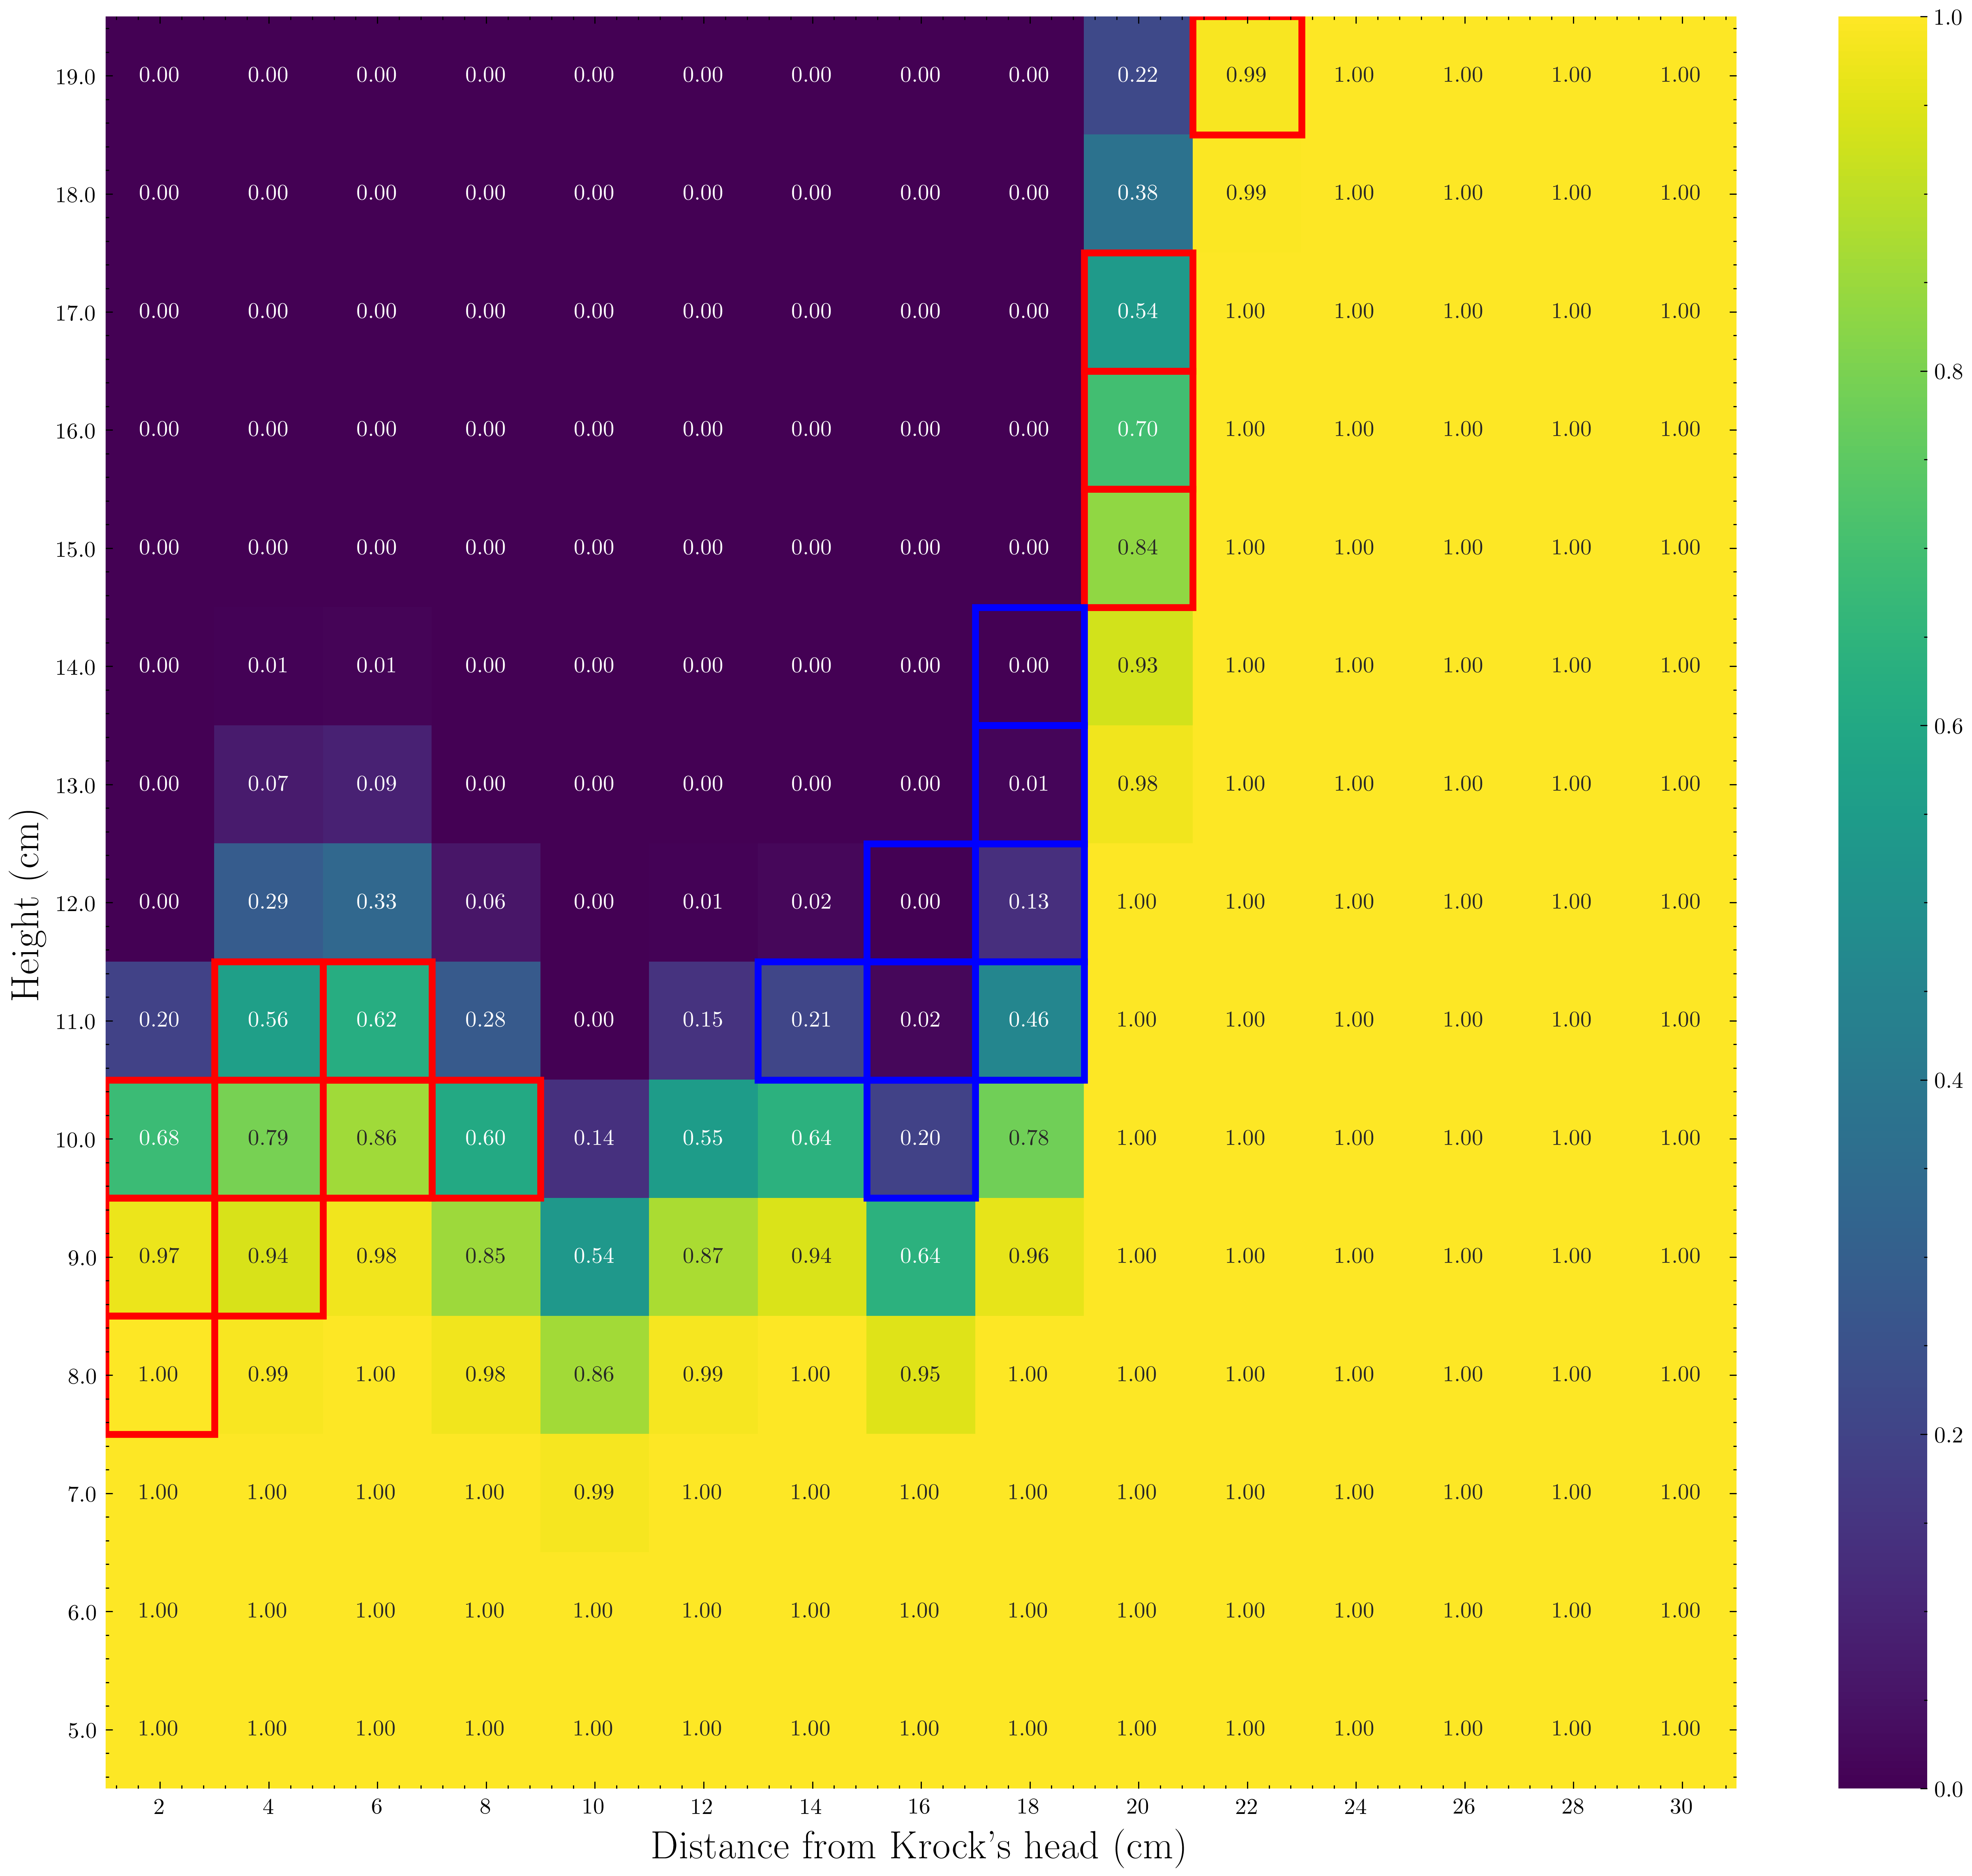
\includegraphics[width=\linewidth]{../img/5/custom_patches/walls_heights/walls_heights_preds.png}
        \caption{Predictions}
        \label{fig : walls-heights-preds}
    \end{subfigure}   
    \begin{subfigure}[b]{0.48\linewidth}
        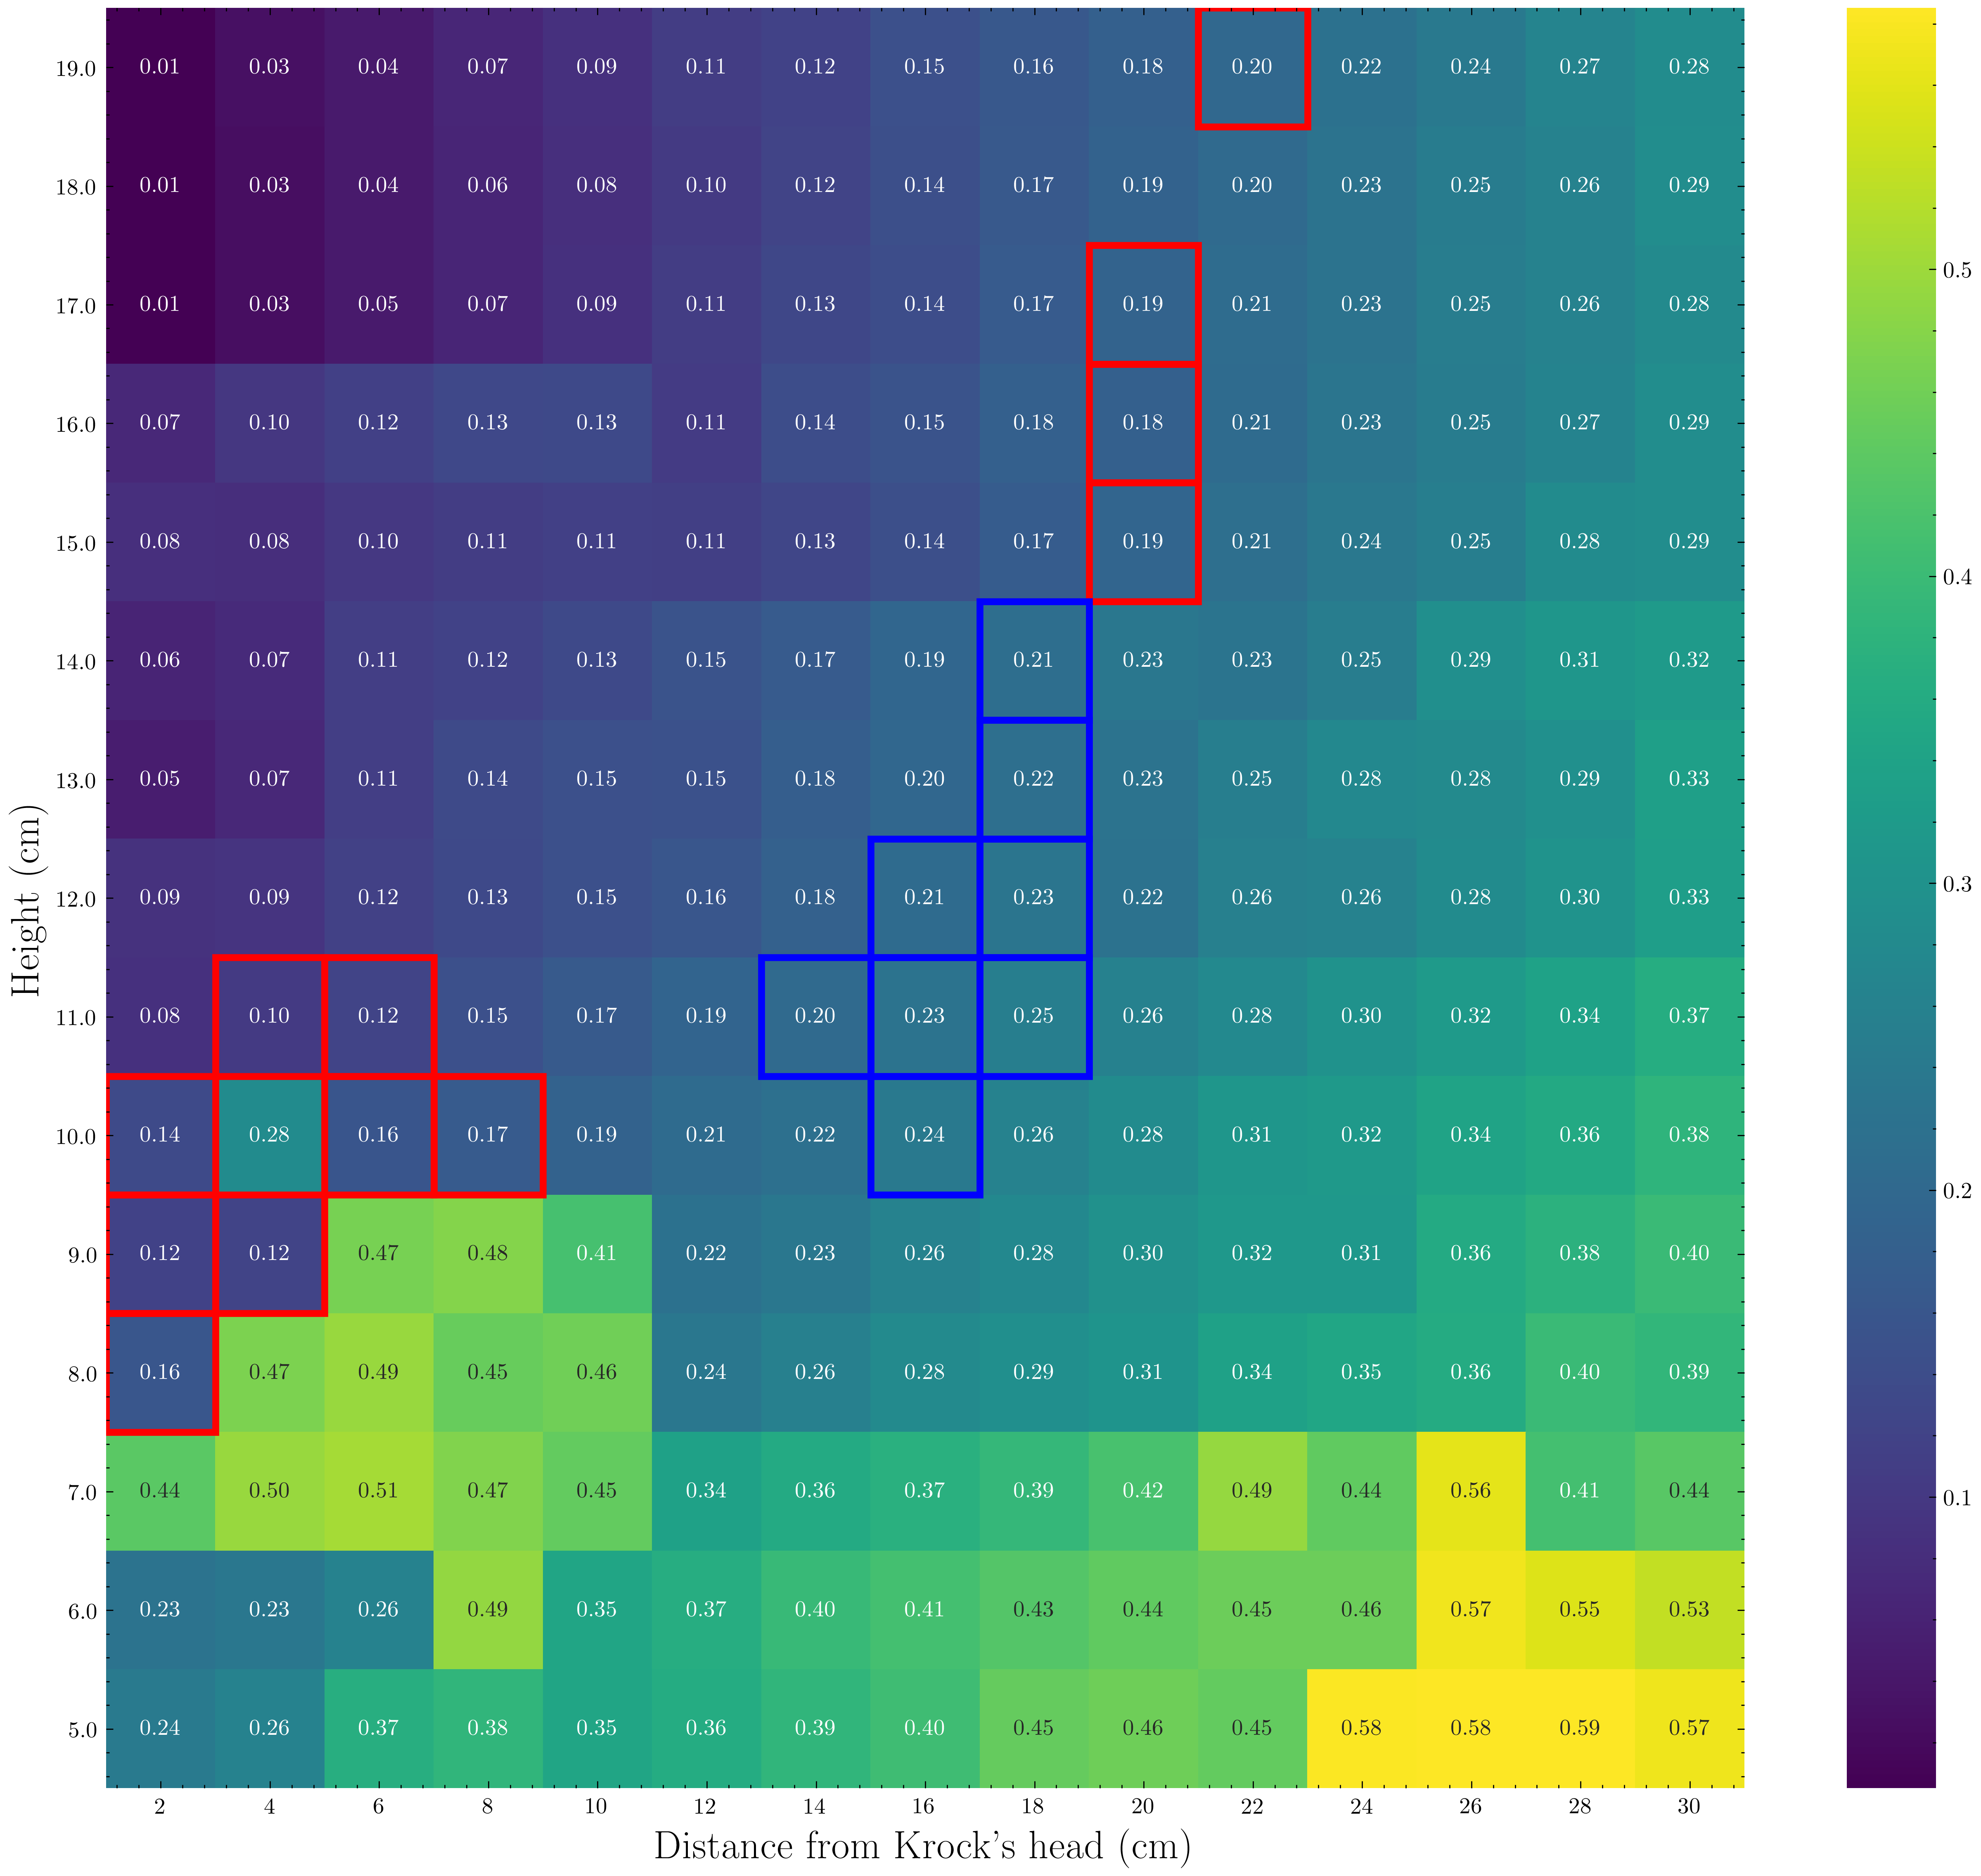
\includegraphics[width=\linewidth]{../img/5/custom_patches/walls_heights/walls_heights_advs.png}
        \caption{Averaged real advancement}
        \label{fig : walls-heights-advs}
    \end{subfigure}   
    \begin{subfigure}[b]{0.48\linewidth}
        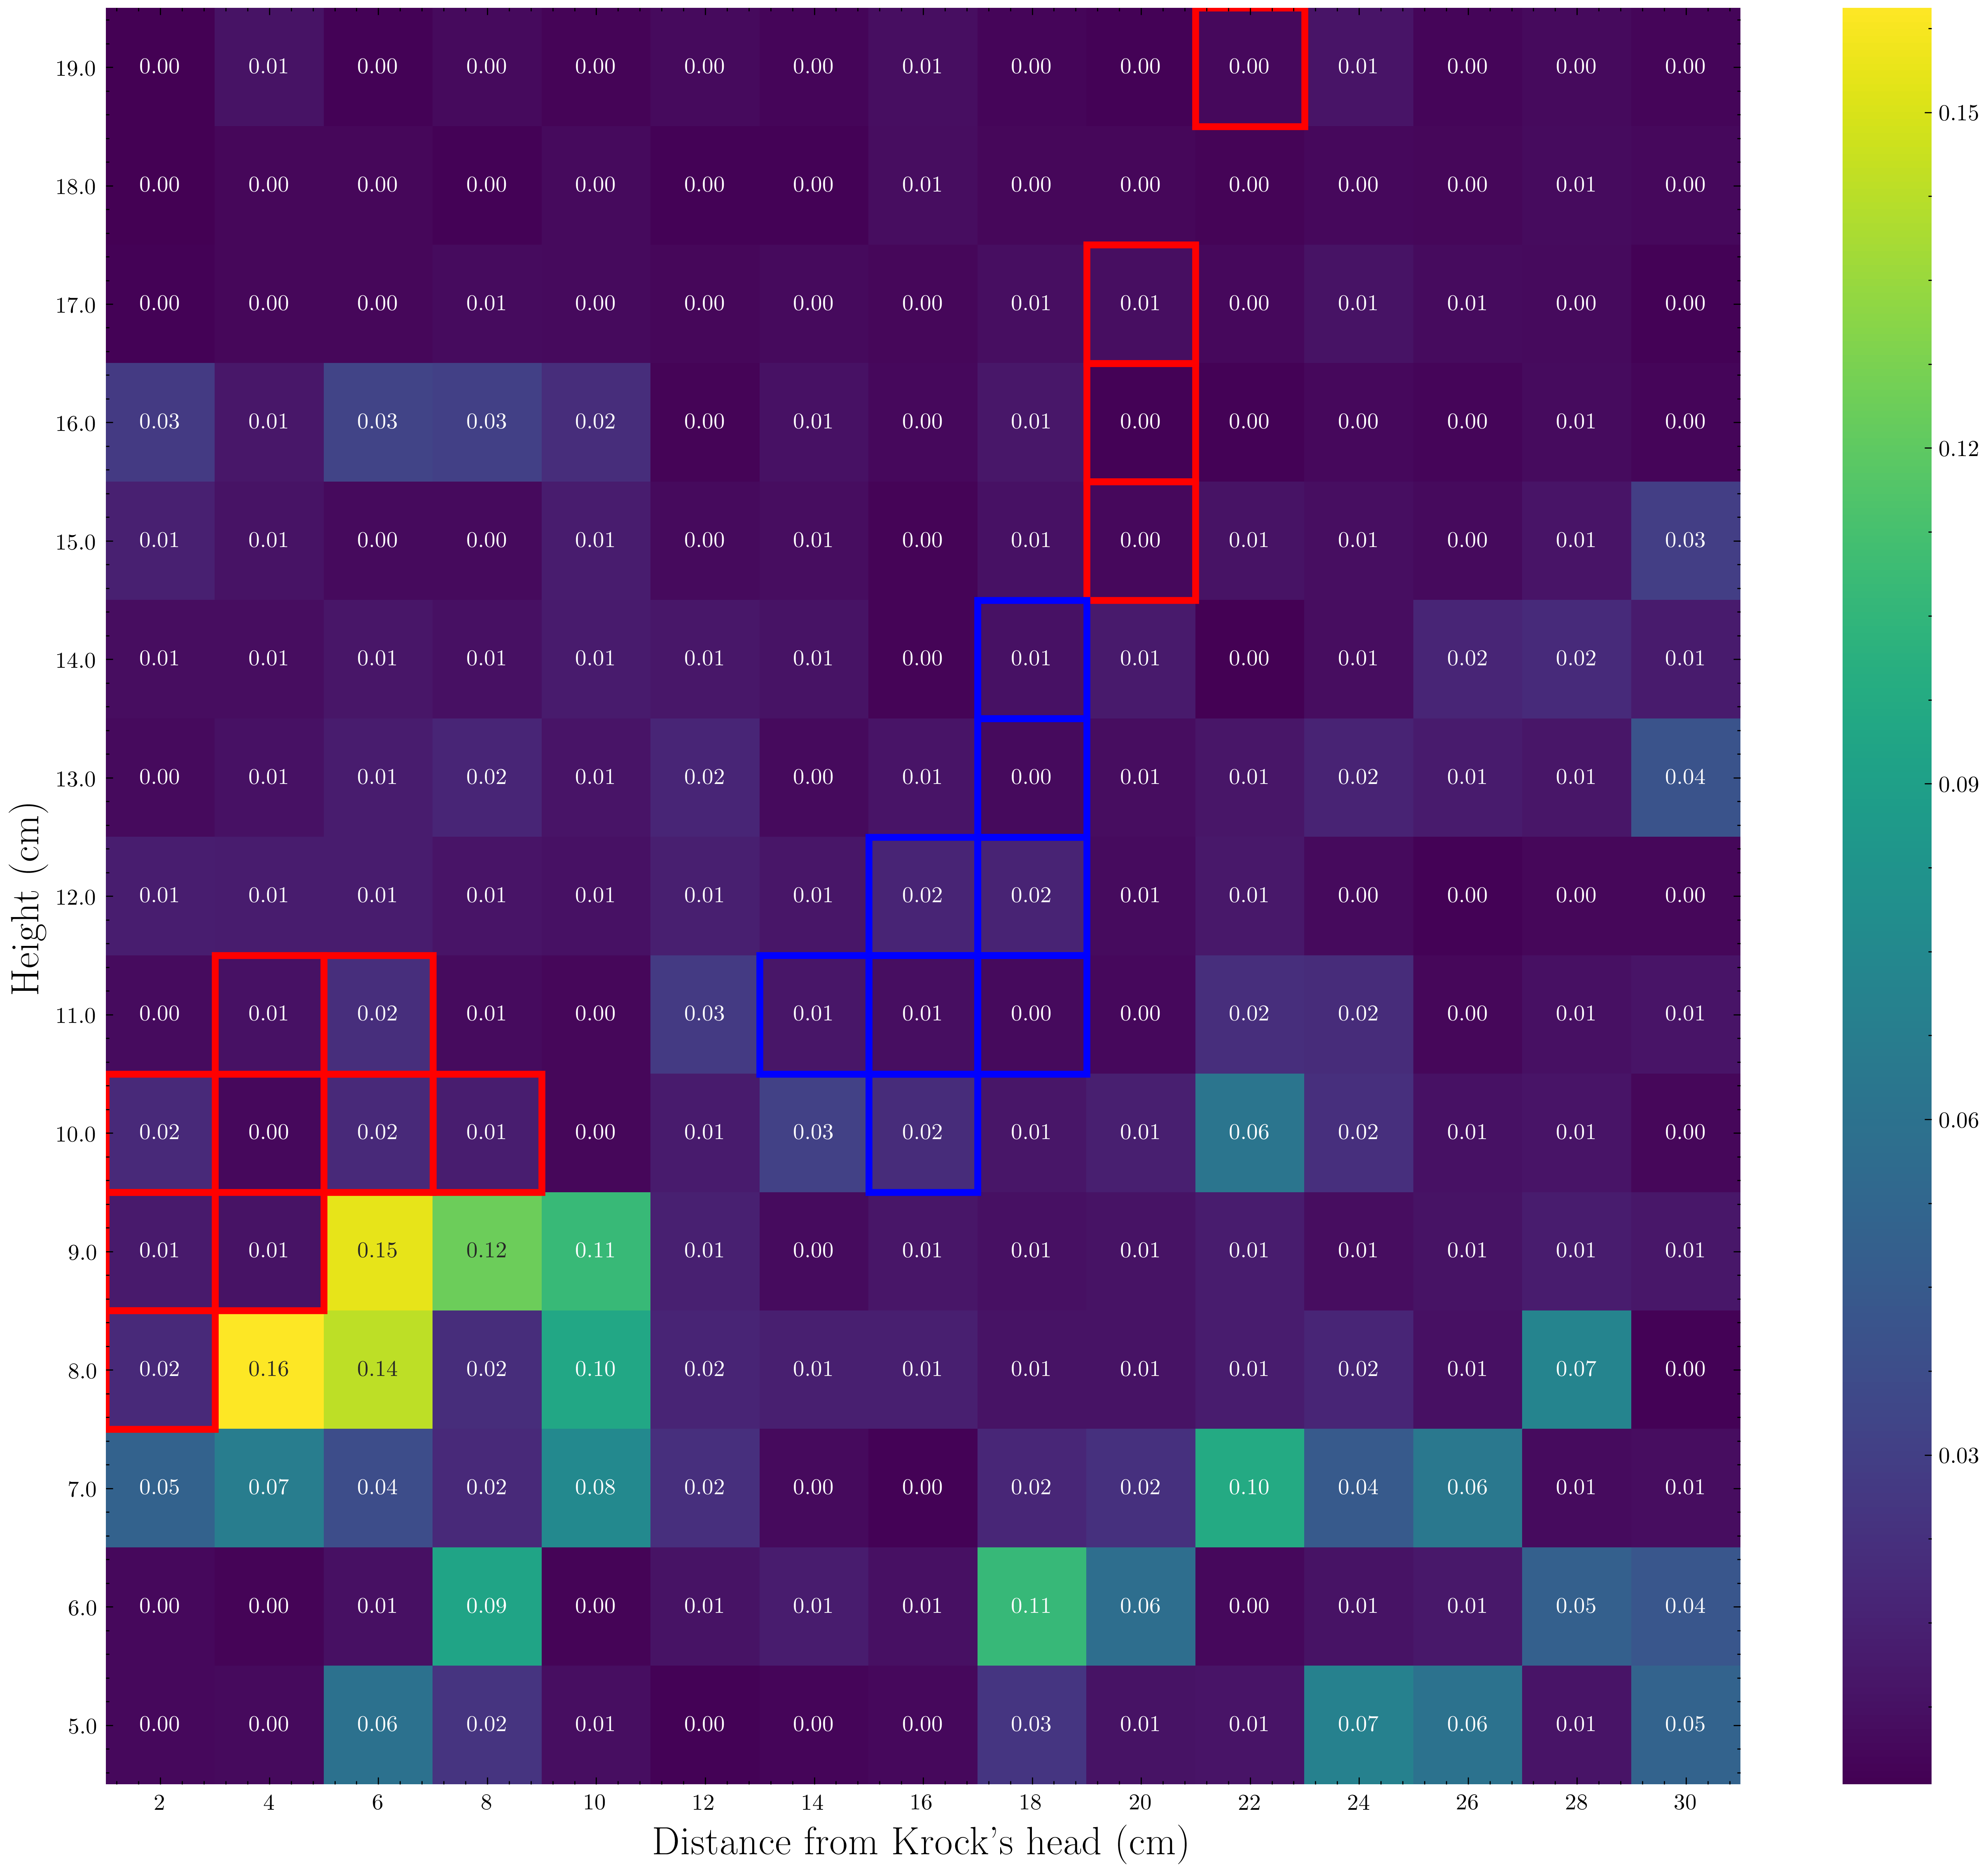
\includegraphics[width=\linewidth]{../img/5/custom_patches/walls_heights/walls_heights_std.png}
        \caption{Standard deviation of the real advancement across six different runs.}
        \label{fig : walls-heights-std}
    \end{subfigure}   
\caption{Results for all the combination of patches with a wall's distance from $2-30$cm and heights between $5 - 19$cm. False negatives are labeled with red while false positive with blue. The model failed to classify some edges cases when the wall is very close to Krock's head and when the wall's distance is near the threshold. The overall accuracy is $91\%$.}    
\label{fig : walls-heights}
\end{figure}
We obtained an overall accuracy of $91\%$. The model failed to predict some of the edge cases. The false positives are located in two regions: on the bottom left and on the top center. The first ones are the patches with a wall just ahead Krock of heights between $\approx 8 - 11$. The second region appears when the wall is at $\approx 20$cm, the threshold. But, even if the model failed to classify those inputs, it shows a correct degree of uncertainty. For example, most of predictions' probability for the patches at $10$cm close to the robot are less than $0.9$, some of them even close to $0.5$.

The false negative, in the middle, are the inputs at distance close to the threshold and with a wall height between traversable and not traversable. Even if the model wrongly classified some of the inputs, all those errors are in the edge cases where the predicted classes' probability is not maximum. Moreover, in most cases, the model's showed uncertainty, especially on the false negative. Also, the prediction changes smoothly without any spikes accordingly to the features of the terrain. This shows a correct degree of understanding of the surface inputs. For instance, If the model outputs not traversable at height of $10$cm and at a distance of $16$cm, then all the taller wall are correctly labeled as not traversable showing consistency and predictability. 
\subsection{Tunnel}
We also tested the model against tunnels. We expected the model to not perform well since in the train set samples with tunnels. The only two maps in the all dataset with possible tunnels, depending on the robot's orientation,  \emph{bars1} and \emph{bars2}. Also, by looking at the different patches plotted in the features space, figure \ref{fig : pca-patches-200}, there only a few patches with tunnels. We generated ten different terrains starting from two walls at $30$cm from the borders. Figure visualize the inputs \ref{fig : tunnels}. 
\begin{figure}[htbp]
    \centering
    \begin{subfigure}[b]{0.24\textwidth}
    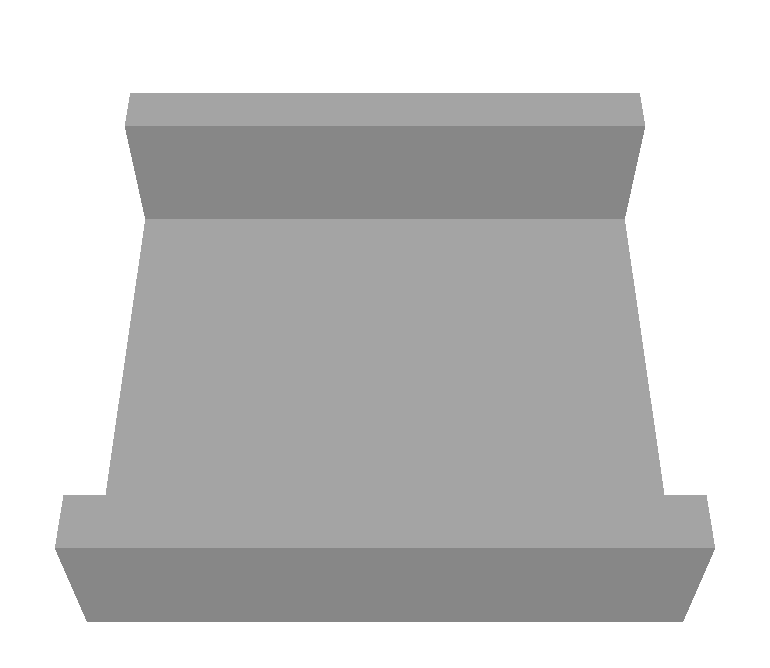
\includegraphics[width=\linewidth]{../img/5/custom_patches/tunnel/all/00-3d.png}
    \end{subfigure}
    \begin{subfigure}[b]{0.24\textwidth}
    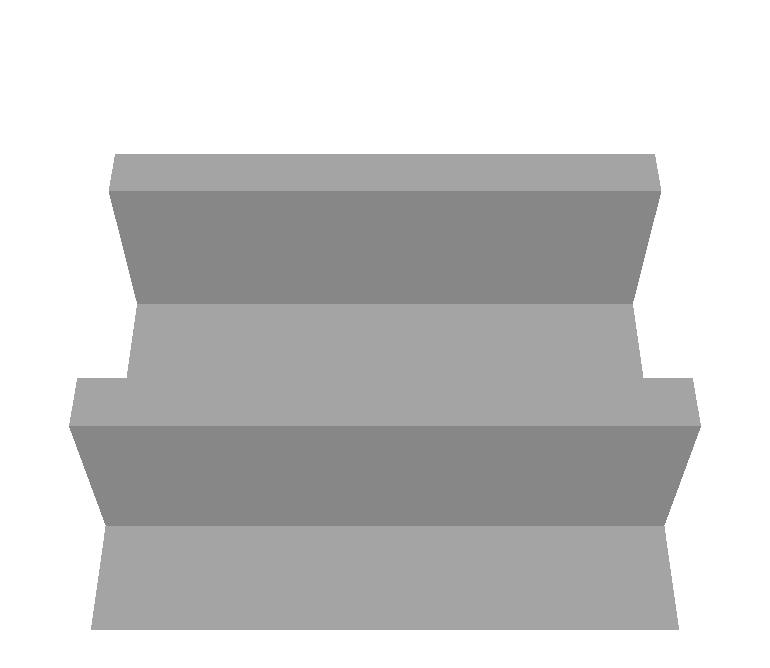
\includegraphics[width=\linewidth]{../img/5/custom_patches/tunnel/all/01-3d.png}
    \end{subfigure}
    \begin{subfigure}[b]{0.24\textwidth}
    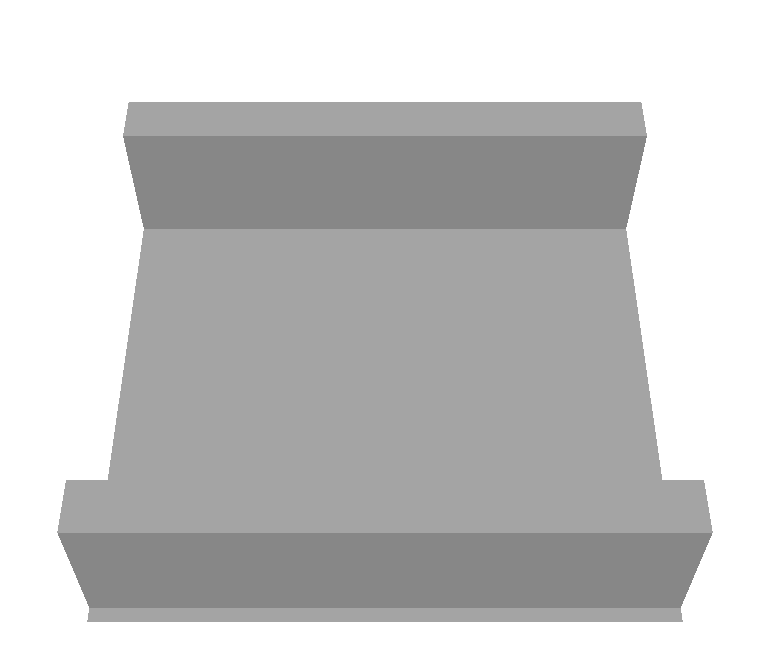
\includegraphics[width=\linewidth]{../img/5/custom_patches/tunnel/all/02-3d.png}
    \end{subfigure}
    \begin{subfigure}[b]{0.24\textwidth}
    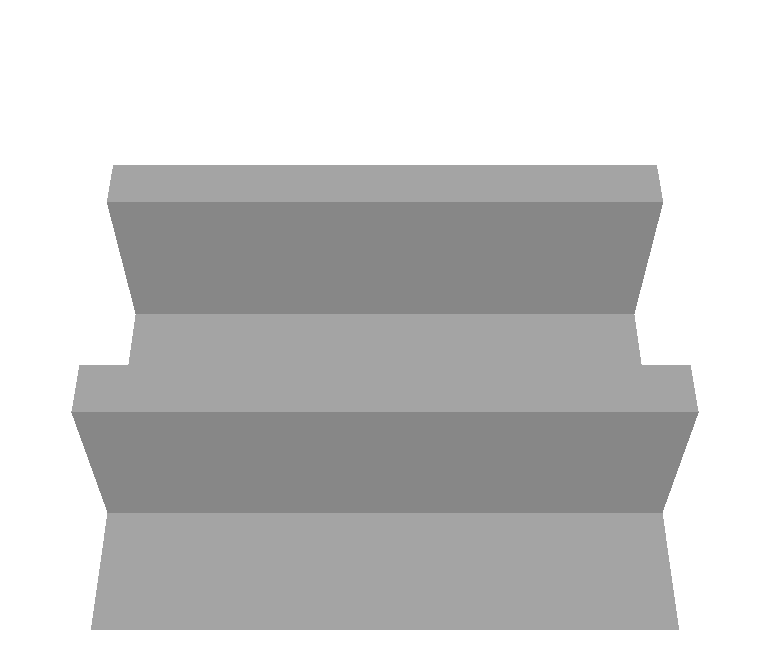
\includegraphics[width=\linewidth]{../img/5/custom_patches/tunnel/all/03-3d.png}
    \end{subfigure}
    \begin{subfigure}[b]{0.24\textwidth}
    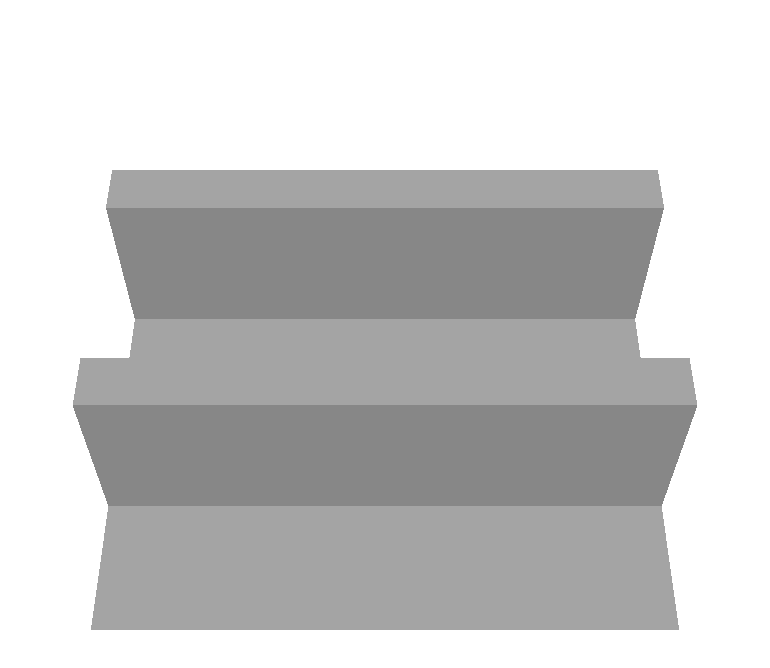
\includegraphics[width=\linewidth]{../img/5/custom_patches/tunnel/all/04-3d.png}
    \end{subfigure}
    \begin{subfigure}[b]{0.24\textwidth}
    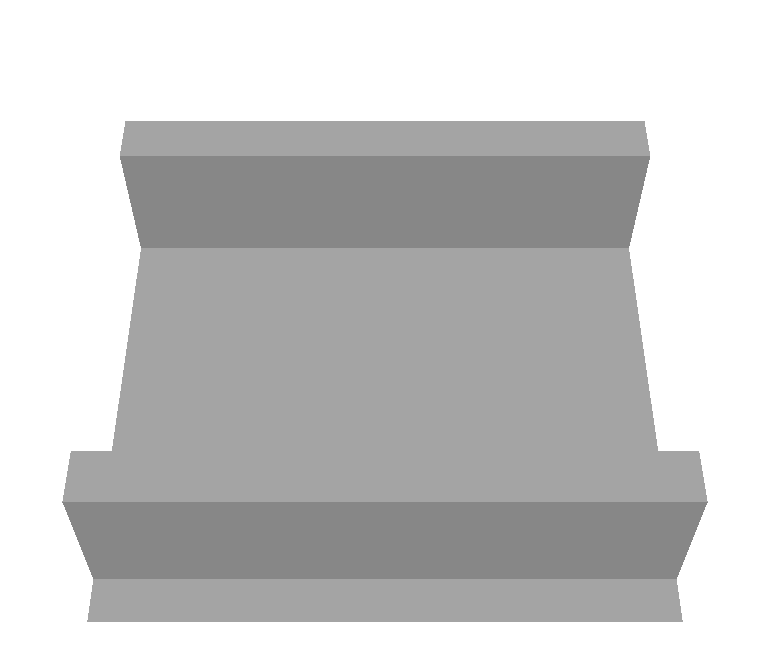
\includegraphics[width=\linewidth]{../img/5/custom_patches/tunnel/all/06-3d.png}
    \end{subfigure}
    \begin{subfigure}[b]{0.24\textwidth}
    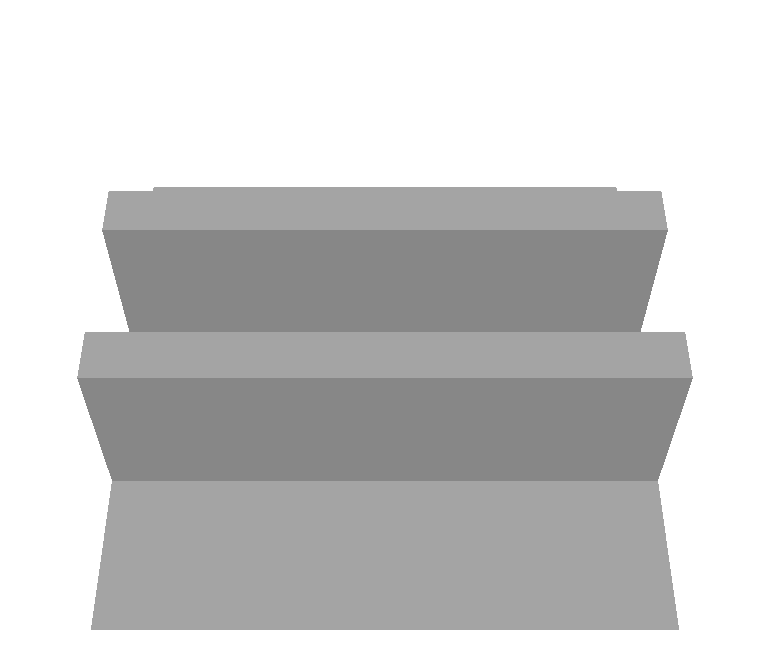
\includegraphics[width=\linewidth]{../img/5/custom_patches/tunnel/all/08-3d.png}
    \end{subfigure}
    \begin{subfigure}[b]{0.24\textwidth}
    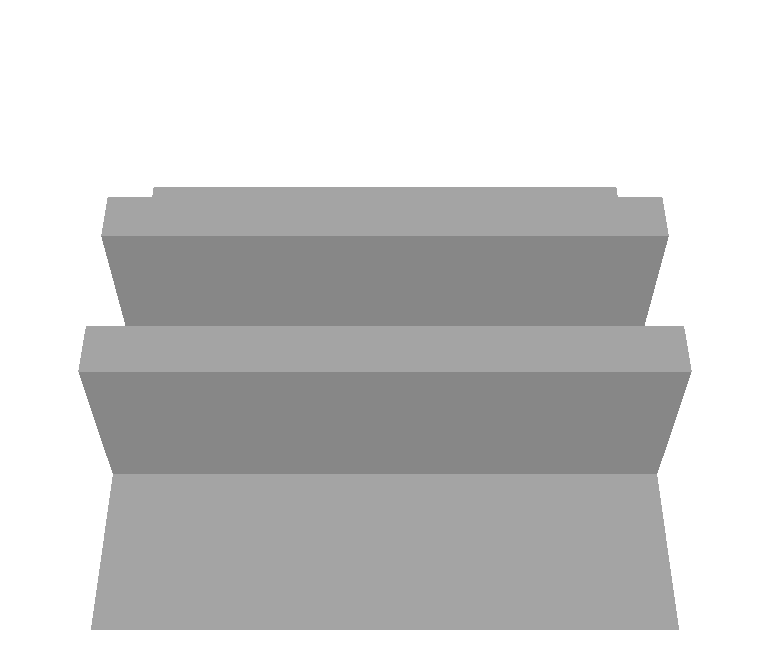
\includegraphics[width=\linewidth]{../img/5/custom_patches/tunnel/all/09-3d.png}
    \end{subfigure}
    \caption{Some of the tested patches with tunnel at different distances.}
    \label{fig : tunnels}
\end{figure}
The model predicted that all patches expect the las two are traversable, figure \ref{tunnels-preds}. 
\begin{figure}[htbp]
    \centering
\begin{subfigure}[b]{1\textwidth}
    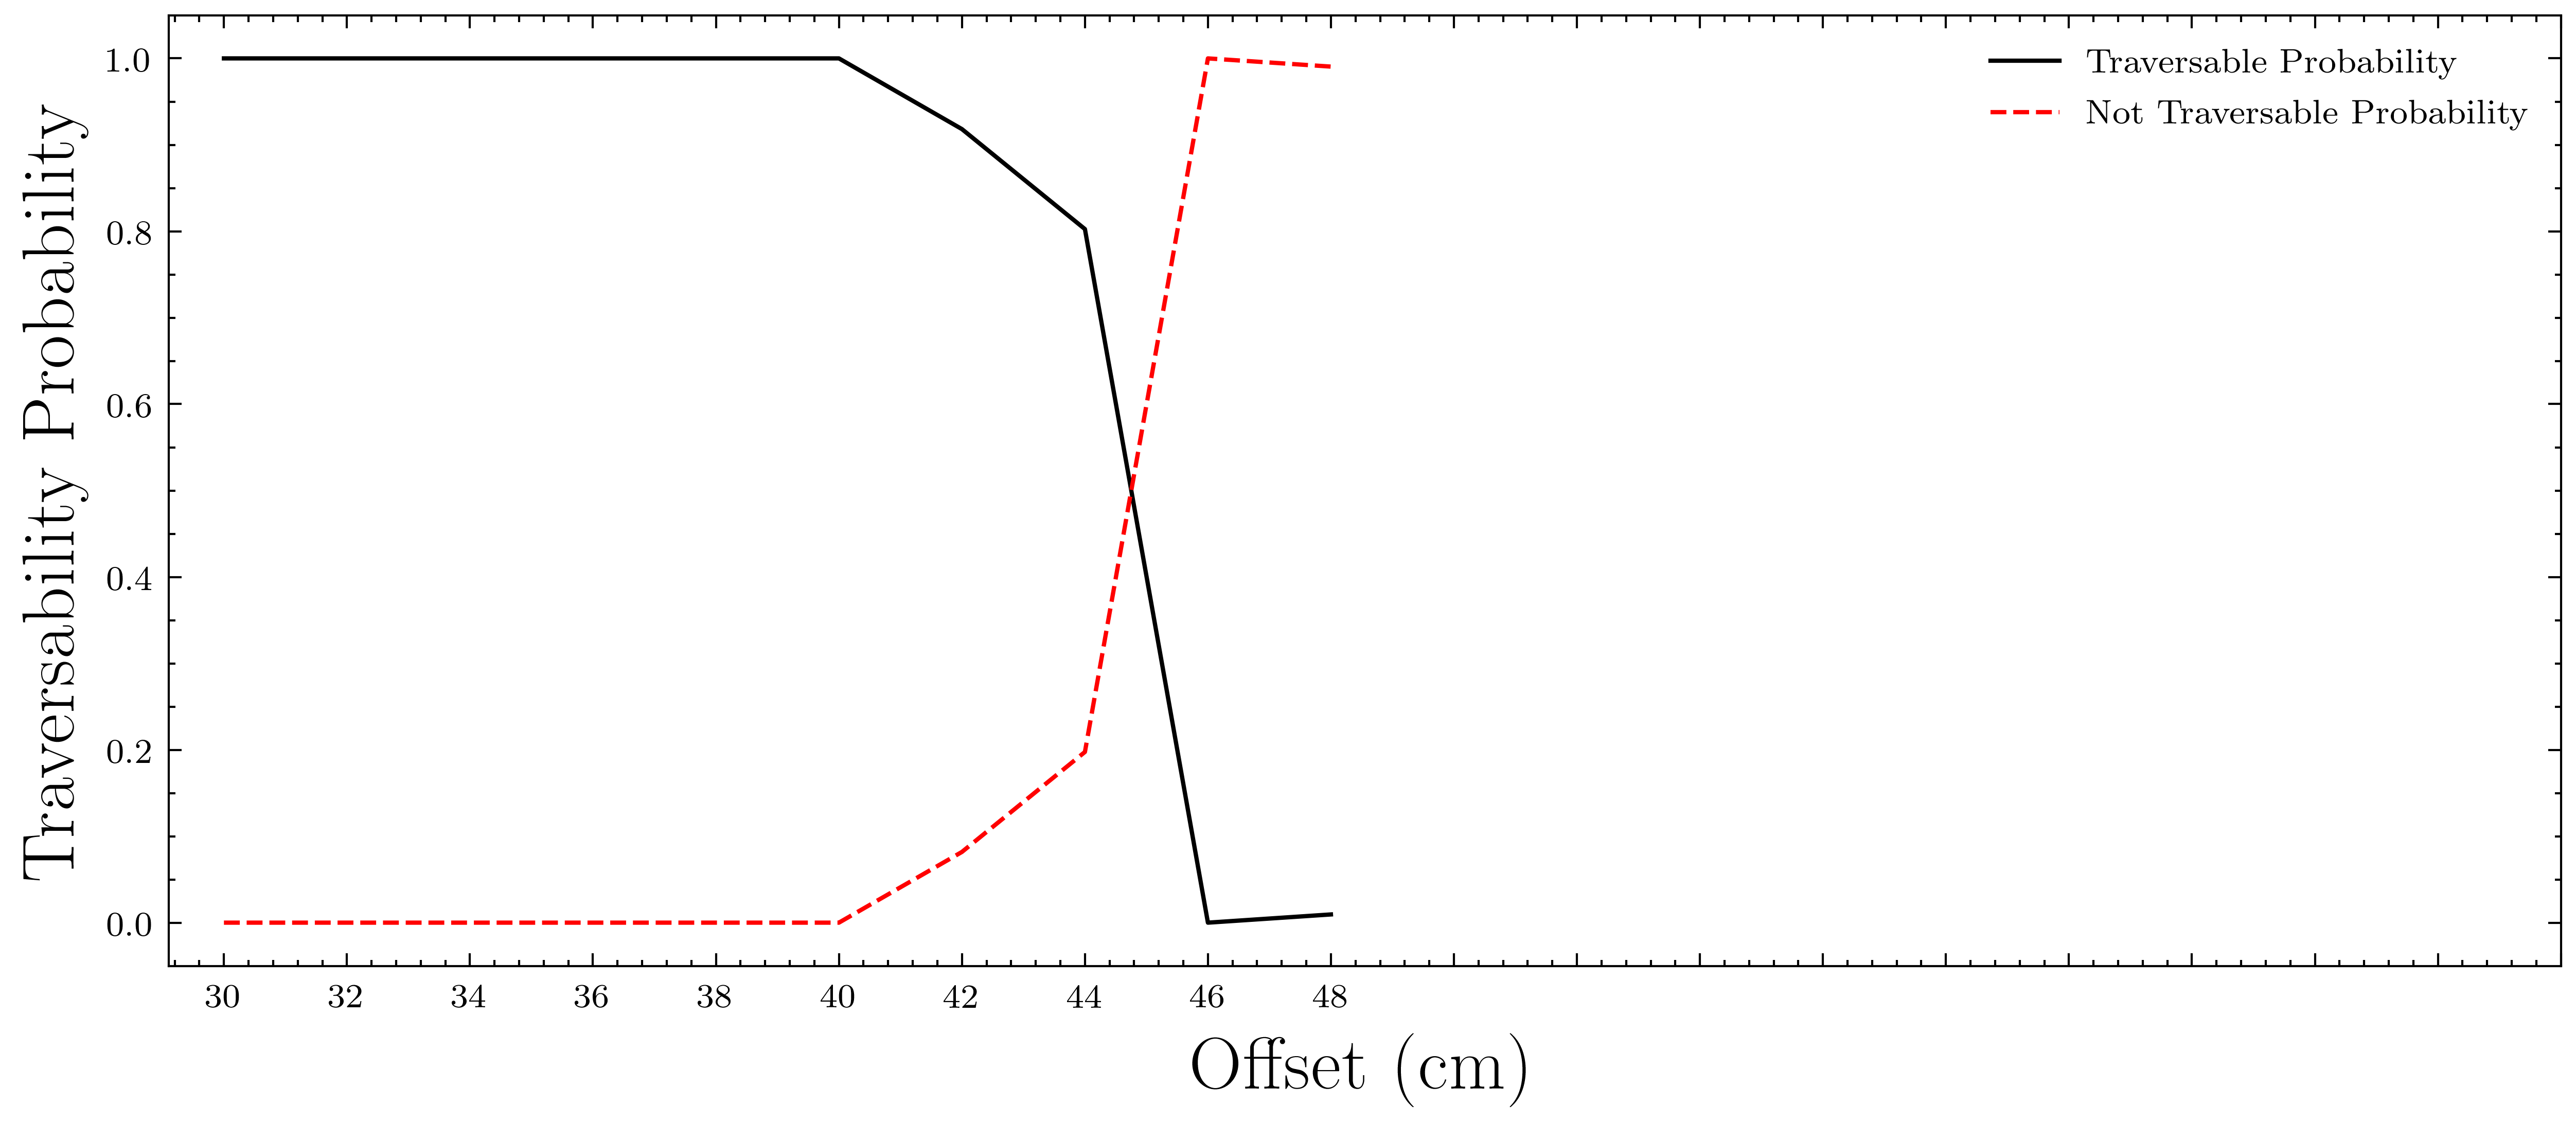
\includegraphics[width=\linewidth]{../img/5/custom_patches/tunnel/predictions.png}
    \end{subfigure}
    \caption{Traversability probabilities against tunnel offset from the top borders..}
    \label{fig: tunnels-preds}
\end{figure}
Unfortunately, after comparing the real data from the simulator, the model scored an accuracy of just $40\%$. Only the first two patches are traversable, while all the others are not. When the distance between the walls reach a certain point, the robot was stuck and it was not able to move. Interesting, all the patches with a space inside the tunnel smaller than Krock's footprint, the last four samples, represented an impossible situation, since in real life the robot cannot go inside an obstacle. But, even some of those inputs were classified as traversable by the model. We utilized Grad-CAM to further investigate what the model is looking in those unrealistic patches. Figure \ref{fig : tunnels-grad-cam} visualize the Grad-CAM directly on them. In the first two, were the model predicted traversable but the distance between the walls is less than the robot's footprint, the front region was highlighted meaning that the network did not consider the distance between the walls, while in the last two patches, the spot corresponding to the robot placement is highlighted. However, the model was clearly confused. This can be solved by incorporating in the train set samples with tunnels.
 \begin{figure}[htbp]
    \centering
    \begin{subfigure}[b]{0.24\textwidth}
    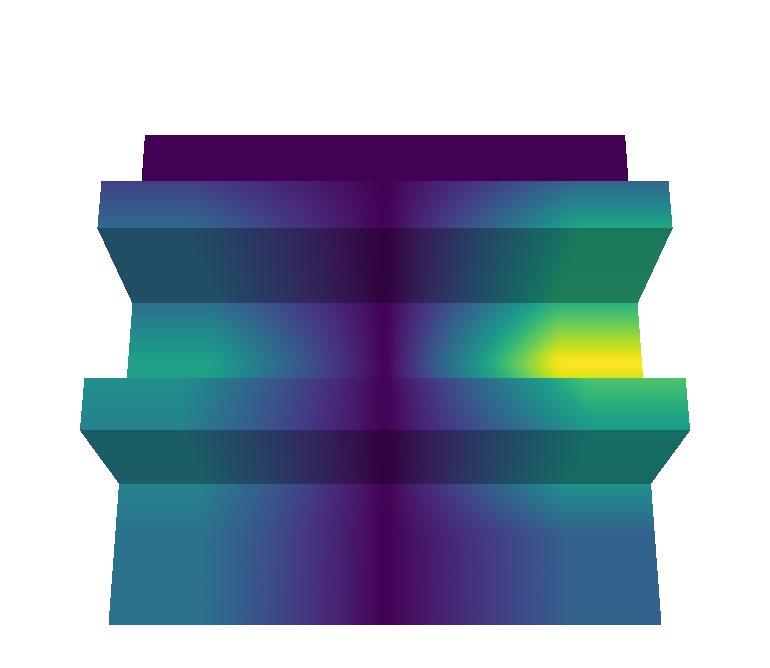
\includegraphics[width=\linewidth]{../img/5/custom_patches/tunnel/all/06-3d-grad.png}
    \end{subfigure}
    \begin{subfigure}[b]{0.24\textwidth}
    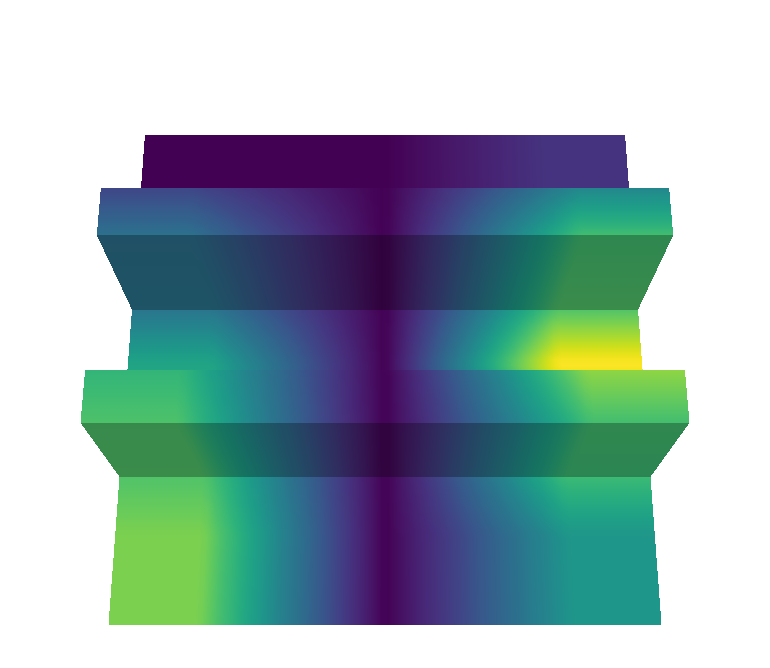
\includegraphics[width=\linewidth]{../img/5/custom_patches/tunnel/all/07-3d-grad.png}
    \end{subfigure}
    \begin{subfigure}[b]{0.24\textwidth}
    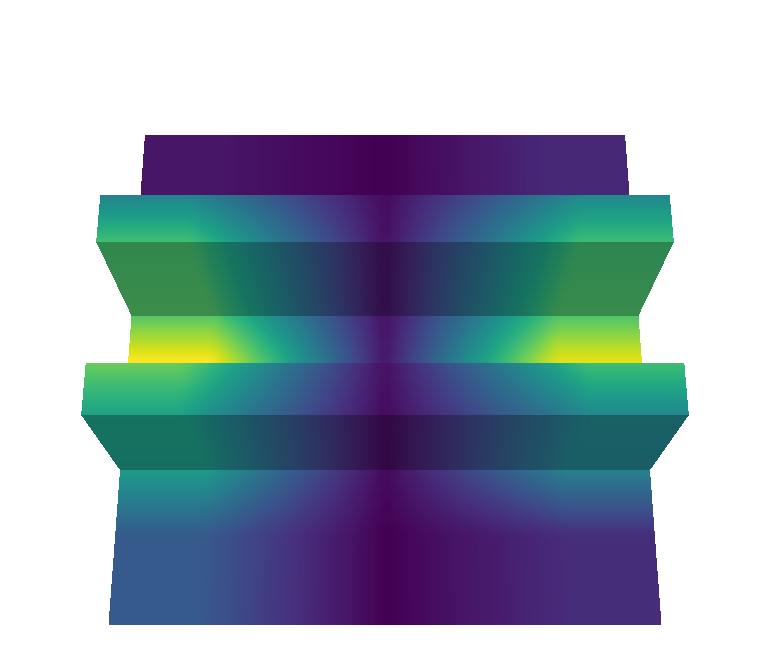
\includegraphics[width=\linewidth]{../img/5/custom_patches/tunnel/all/08-3d-grad.png}
    \end{subfigure}
    \begin{subfigure}[b]{0.24\textwidth}
    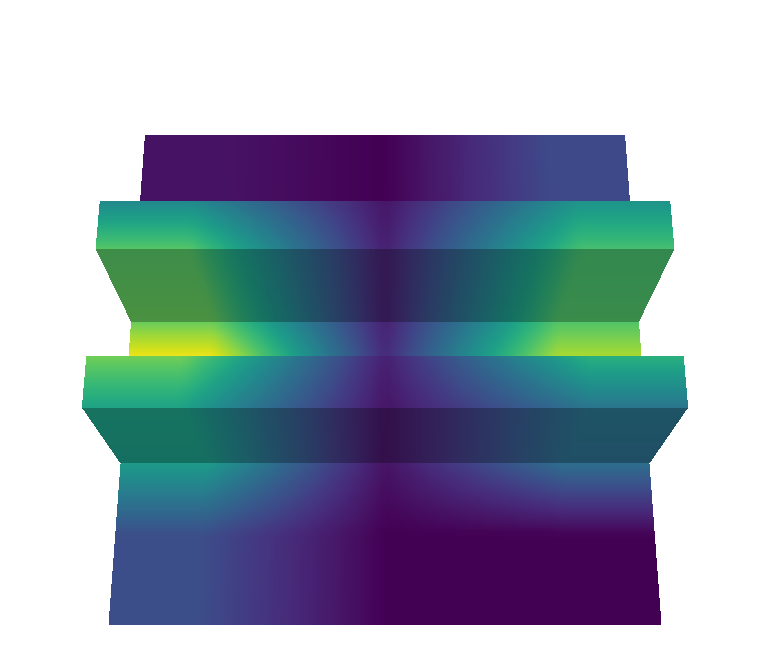
\includegraphics[width=\linewidth]{../img/5/custom_patches/tunnel/all/09-3d-grad.png}
    \end{subfigure}
    \caption{Fours patches with the distance between the wall smaller than Krock's footprint making impossible for the robot traverse them. Only the last to surfaces were correct label as not traversable.}
    \label{fig : tunnels-grad-cam}
\end{figure}
\subsection{Ramps}
Using the same methodology from the last sections, we generated twenty ramps with a maximum height from $0.25$m to $4$m. Figure \ref{fig: ramps} shows some of the inputs. The model labeled as traversable the surfaces with a maximum height less than $1$m and not traversable the others, figure \ref{fig : ramps-preds} plots the traversability probabilities against the maximum height of each ramp. Then, we tested the last traversable patch and the first not traversable with the real advancement gather from the simulator. Figure \ref{fig : ramps-sim} shows that the model's predictions are confirmed by the ground truth values. 
\begin{figure}[htbp]
    \centering
    \begin{subfigure}[b]{0.24\textwidth}
    
\includegraphics[width=\linewidth]{../img/5/custom_patches/ramp/all/00-3d.png}
    \end{subfigure}
    \begin{subfigure}[b]{0.24\textwidth}
    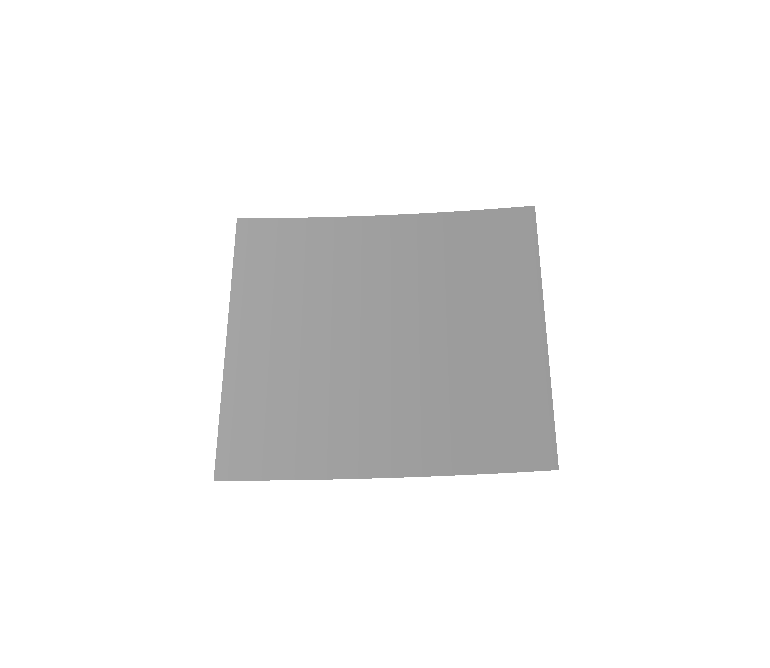
\includegraphics[width=\linewidth]{../img/5/custom_patches/ramp/all/03-3d.png}
    \end{subfigure}
    \begin{subfigure}[b]{0.24\textwidth}
    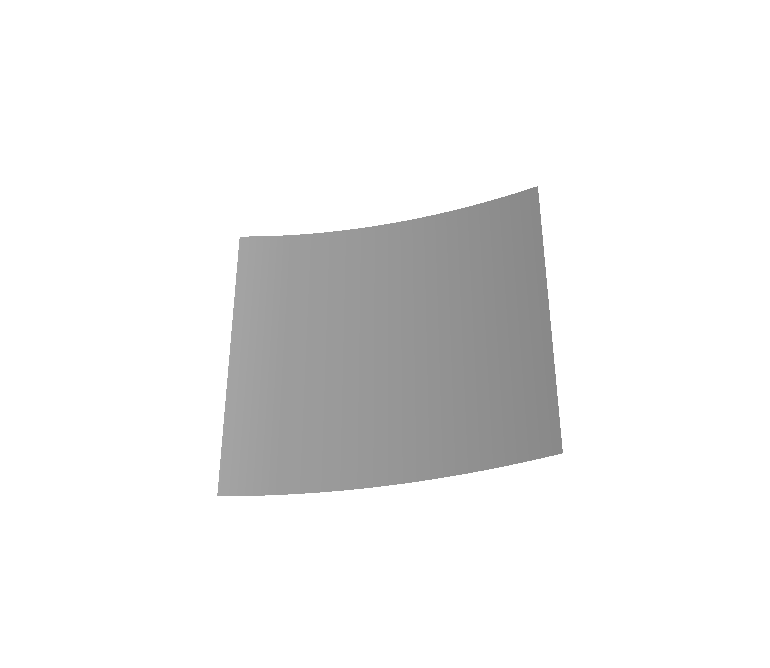
\includegraphics[width=\linewidth]{../img/5/custom_patches/ramp/all/06-3d.png}
    \end{subfigure}
    \begin{subfigure}[b]{0.24\textwidth}
    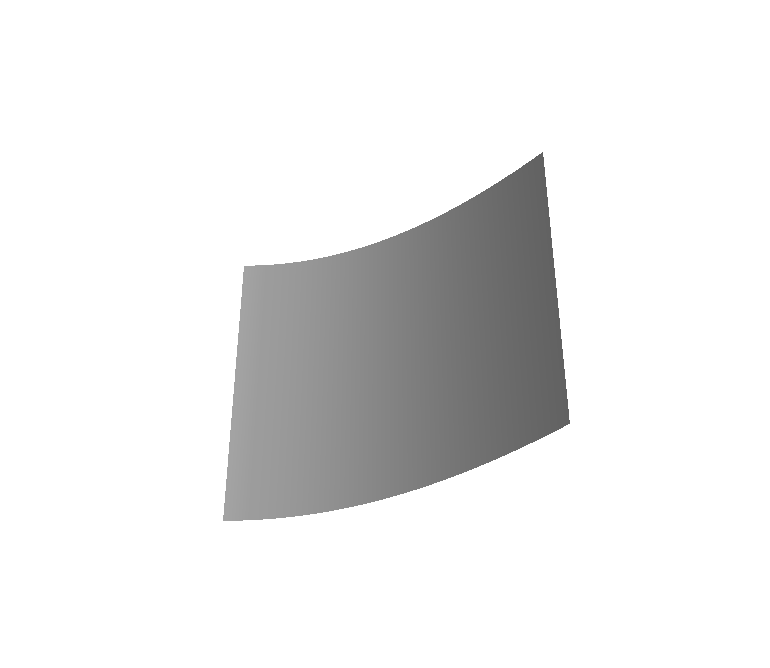
\includegraphics[width=\linewidth]{../img/5/custom_patches/ramp/all/09-3d.png}
    \end{subfigure}
    \begin{subfigure}[b]{0.24\textwidth}
    
\includegraphics[width=\linewidth]{../img/5/custom_patches/ramp/all/11-3d.png}
    \end{subfigure}
    \begin{subfigure}[b]{0.24\textwidth}
    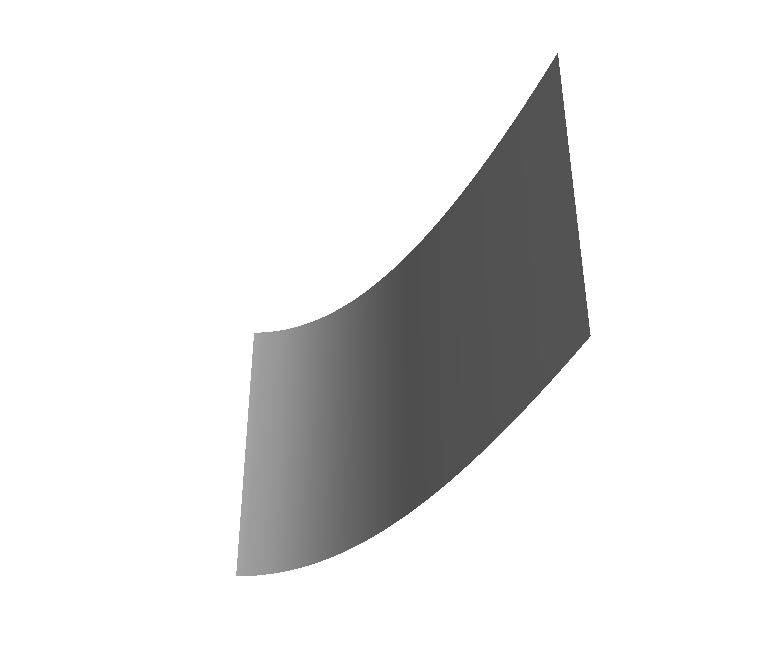
\includegraphics[width=\linewidth]{../img/5/custom_patches/ramp/all/14-3d.png}
    \end{subfigure}
    \begin{subfigure}[b]{0.24\textwidth}
    \includegraphics[width=\linewidth]{../img/5/custom_patches/ramp/all/17-3d.png}
    \end{subfigure}
    \begin{subfigure}[b]{0.24\textwidth}
    \includegraphics[width=\linewidth]{../img/5/custom_patches/ramp/all/19-3d.png}
    \end{subfigure}
    \caption{Some of the tested patches with steep ramps.}
    \label{fig: ramps}
    \end{figure}
\begin{figure}[htbp]
    \centering
    \begin{subfigure}[b]{1\textwidth}
    \includegraphics[width=\linewidth]{../img/5/custom_patches/ramp/predictions.png}
    \end{subfigure}
    \caption{Traversability probabilities against maximum height of each ramp.}
    \label{fig: ramps-preds}
\end{figure}
\begin{figure}[htbp]
    \centering
    \begin{subfigure}[b]{0.33\textwidth}
        \includegraphics[width=\linewidth]{../img/5/custom_patches/ramp/ramp-6-2d.png}
    \end{subfigure}   
    \begin{subfigure}[b]{0.33\textwidth}
        \includegraphics[width=\linewidth]{../img/5/custom_patches/ramp/ramp-7-2d}
    \end{subfigure}   
    \begin{subfigure}[b]{0.33\textwidth}
        \includegraphics[width=\linewidth]{../img/5/custom_patches/ramp/ramp-6-3d.png}
    \caption{Height $0.94$cm}
    \end{subfigure}   
    \begin{subfigure}[b]{0.33\textwidth}
        \includegraphics[width=\linewidth]{../img/5/custom_patches/ramp/ramp-7-3d}
        \caption{height $1.1$m}
    \end{subfigure}   
\caption{The last traversable and the first non traversable patches with a steep ramp ahead of Krock.}    
\label{fig: ramps-sim}
\end{figure}
\end{document}